% Options for packages loaded elsewhere
\PassOptionsToPackage{unicode}{hyperref}
\PassOptionsToPackage{hyphens}{url}
\PassOptionsToPackage{dvipsnames,svgnames,x11names}{xcolor}
%
\documentclass[
  letterpaper,
  DIV=11,
  numbers=noendperiod]{scrartcl}

\usepackage{amsmath,amssymb}
\usepackage{iftex}
\ifPDFTeX
  \usepackage[T1]{fontenc}
  \usepackage[utf8]{inputenc}
  \usepackage{textcomp} % provide euro and other symbols
\else % if luatex or xetex
  \usepackage{unicode-math}
  \defaultfontfeatures{Scale=MatchLowercase}
  \defaultfontfeatures[\rmfamily]{Ligatures=TeX,Scale=1}
\fi
\usepackage{lmodern}
\ifPDFTeX\else  
    % xetex/luatex font selection
\fi
% Use upquote if available, for straight quotes in verbatim environments
\IfFileExists{upquote.sty}{\usepackage{upquote}}{}
\IfFileExists{microtype.sty}{% use microtype if available
  \usepackage[]{microtype}
  \UseMicrotypeSet[protrusion]{basicmath} % disable protrusion for tt fonts
}{}
\makeatletter
\@ifundefined{KOMAClassName}{% if non-KOMA class
  \IfFileExists{parskip.sty}{%
    \usepackage{parskip}
  }{% else
    \setlength{\parindent}{0pt}
    \setlength{\parskip}{6pt plus 2pt minus 1pt}}
}{% if KOMA class
  \KOMAoptions{parskip=half}}
\makeatother
\usepackage{xcolor}
\setlength{\emergencystretch}{3em} % prevent overfull lines
\setcounter{secnumdepth}{-\maxdimen} % remove section numbering
% Make \paragraph and \subparagraph free-standing
\ifx\paragraph\undefined\else
  \let\oldparagraph\paragraph
  \renewcommand{\paragraph}[1]{\oldparagraph{#1}\mbox{}}
\fi
\ifx\subparagraph\undefined\else
  \let\oldsubparagraph\subparagraph
  \renewcommand{\subparagraph}[1]{\oldsubparagraph{#1}\mbox{}}
\fi

\usepackage{color}
\usepackage{fancyvrb}
\newcommand{\VerbBar}{|}
\newcommand{\VERB}{\Verb[commandchars=\\\{\}]}
\DefineVerbatimEnvironment{Highlighting}{Verbatim}{commandchars=\\\{\}}
% Add ',fontsize=\small' for more characters per line
\usepackage{framed}
\definecolor{shadecolor}{RGB}{241,243,245}
\newenvironment{Shaded}{\begin{snugshade}}{\end{snugshade}}
\newcommand{\AlertTok}[1]{\textcolor[rgb]{0.68,0.00,0.00}{#1}}
\newcommand{\AnnotationTok}[1]{\textcolor[rgb]{0.37,0.37,0.37}{#1}}
\newcommand{\AttributeTok}[1]{\textcolor[rgb]{0.40,0.45,0.13}{#1}}
\newcommand{\BaseNTok}[1]{\textcolor[rgb]{0.68,0.00,0.00}{#1}}
\newcommand{\BuiltInTok}[1]{\textcolor[rgb]{0.00,0.23,0.31}{#1}}
\newcommand{\CharTok}[1]{\textcolor[rgb]{0.13,0.47,0.30}{#1}}
\newcommand{\CommentTok}[1]{\textcolor[rgb]{0.37,0.37,0.37}{#1}}
\newcommand{\CommentVarTok}[1]{\textcolor[rgb]{0.37,0.37,0.37}{\textit{#1}}}
\newcommand{\ConstantTok}[1]{\textcolor[rgb]{0.56,0.35,0.01}{#1}}
\newcommand{\ControlFlowTok}[1]{\textcolor[rgb]{0.00,0.23,0.31}{#1}}
\newcommand{\DataTypeTok}[1]{\textcolor[rgb]{0.68,0.00,0.00}{#1}}
\newcommand{\DecValTok}[1]{\textcolor[rgb]{0.68,0.00,0.00}{#1}}
\newcommand{\DocumentationTok}[1]{\textcolor[rgb]{0.37,0.37,0.37}{\textit{#1}}}
\newcommand{\ErrorTok}[1]{\textcolor[rgb]{0.68,0.00,0.00}{#1}}
\newcommand{\ExtensionTok}[1]{\textcolor[rgb]{0.00,0.23,0.31}{#1}}
\newcommand{\FloatTok}[1]{\textcolor[rgb]{0.68,0.00,0.00}{#1}}
\newcommand{\FunctionTok}[1]{\textcolor[rgb]{0.28,0.35,0.67}{#1}}
\newcommand{\ImportTok}[1]{\textcolor[rgb]{0.00,0.46,0.62}{#1}}
\newcommand{\InformationTok}[1]{\textcolor[rgb]{0.37,0.37,0.37}{#1}}
\newcommand{\KeywordTok}[1]{\textcolor[rgb]{0.00,0.23,0.31}{#1}}
\newcommand{\NormalTok}[1]{\textcolor[rgb]{0.00,0.23,0.31}{#1}}
\newcommand{\OperatorTok}[1]{\textcolor[rgb]{0.37,0.37,0.37}{#1}}
\newcommand{\OtherTok}[1]{\textcolor[rgb]{0.00,0.23,0.31}{#1}}
\newcommand{\PreprocessorTok}[1]{\textcolor[rgb]{0.68,0.00,0.00}{#1}}
\newcommand{\RegionMarkerTok}[1]{\textcolor[rgb]{0.00,0.23,0.31}{#1}}
\newcommand{\SpecialCharTok}[1]{\textcolor[rgb]{0.37,0.37,0.37}{#1}}
\newcommand{\SpecialStringTok}[1]{\textcolor[rgb]{0.13,0.47,0.30}{#1}}
\newcommand{\StringTok}[1]{\textcolor[rgb]{0.13,0.47,0.30}{#1}}
\newcommand{\VariableTok}[1]{\textcolor[rgb]{0.07,0.07,0.07}{#1}}
\newcommand{\VerbatimStringTok}[1]{\textcolor[rgb]{0.13,0.47,0.30}{#1}}
\newcommand{\WarningTok}[1]{\textcolor[rgb]{0.37,0.37,0.37}{\textit{#1}}}

\providecommand{\tightlist}{%
  \setlength{\itemsep}{0pt}\setlength{\parskip}{0pt}}\usepackage{longtable,booktabs,array}
\usepackage{calc} % for calculating minipage widths
% Correct order of tables after \paragraph or \subparagraph
\usepackage{etoolbox}
\makeatletter
\patchcmd\longtable{\par}{\if@noskipsec\mbox{}\fi\par}{}{}
\makeatother
% Allow footnotes in longtable head/foot
\IfFileExists{footnotehyper.sty}{\usepackage{footnotehyper}}{\usepackage{footnote}}
\makesavenoteenv{longtable}
\usepackage{graphicx}
\makeatletter
\def\maxwidth{\ifdim\Gin@nat@width>\linewidth\linewidth\else\Gin@nat@width\fi}
\def\maxheight{\ifdim\Gin@nat@height>\textheight\textheight\else\Gin@nat@height\fi}
\makeatother
% Scale images if necessary, so that they will not overflow the page
% margins by default, and it is still possible to overwrite the defaults
% using explicit options in \includegraphics[width, height, ...]{}
\setkeys{Gin}{width=\maxwidth,height=\maxheight,keepaspectratio}
% Set default figure placement to htbp
\makeatletter
\def\fps@figure{htbp}
\makeatother

\KOMAoption{captions}{tableheading}
\makeatletter
\makeatother
\makeatletter
\makeatother
\makeatletter
\@ifpackageloaded{caption}{}{\usepackage{caption}}
\AtBeginDocument{%
\ifdefined\contentsname
  \renewcommand*\contentsname{Table of contents}
\else
  \newcommand\contentsname{Table of contents}
\fi
\ifdefined\listfigurename
  \renewcommand*\listfigurename{List of Figures}
\else
  \newcommand\listfigurename{List of Figures}
\fi
\ifdefined\listtablename
  \renewcommand*\listtablename{List of Tables}
\else
  \newcommand\listtablename{List of Tables}
\fi
\ifdefined\figurename
  \renewcommand*\figurename{Figure}
\else
  \newcommand\figurename{Figure}
\fi
\ifdefined\tablename
  \renewcommand*\tablename{Table}
\else
  \newcommand\tablename{Table}
\fi
}
\@ifpackageloaded{float}{}{\usepackage{float}}
\floatstyle{ruled}
\@ifundefined{c@chapter}{\newfloat{codelisting}{h}{lop}}{\newfloat{codelisting}{h}{lop}[chapter]}
\floatname{codelisting}{Listing}
\newcommand*\listoflistings{\listof{codelisting}{List of Listings}}
\makeatother
\makeatletter
\@ifpackageloaded{caption}{}{\usepackage{caption}}
\@ifpackageloaded{subcaption}{}{\usepackage{subcaption}}
\makeatother
\makeatletter
\@ifpackageloaded{tcolorbox}{}{\usepackage[skins,breakable]{tcolorbox}}
\makeatother
\makeatletter
\@ifundefined{shadecolor}{\definecolor{shadecolor}{rgb}{.97, .97, .97}}
\makeatother
\makeatletter
\makeatother
\makeatletter
\makeatother
\ifLuaTeX
  \usepackage{selnolig}  % disable illegal ligatures
\fi
\IfFileExists{bookmark.sty}{\usepackage{bookmark}}{\usepackage{hyperref}}
\IfFileExists{xurl.sty}{\usepackage{xurl}}{} % add URL line breaks if available
\urlstyle{same} % disable monospaced font for URLs
\hypersetup{
  pdftitle={Forecasting the United States' Theoretical Unemployment Rate in the Absence of the Covid-19 Pandemic},
  pdfauthor={Lyndsey Umsted},
  colorlinks=true,
  linkcolor={blue},
  filecolor={Maroon},
  citecolor={Blue},
  urlcolor={Blue},
  pdfcreator={LaTeX via pandoc}}

\title{Forecasting the United States' Theoretical Unemployment Rate in
the Absence of the Covid-19 Pandemic}
\author{Lyndsey Umsted}
\date{}

\begin{document}
\maketitle
\ifdefined\Shaded\renewenvironment{Shaded}{\begin{tcolorbox}[breakable, borderline west={3pt}{0pt}{shadecolor}, sharp corners, boxrule=0pt, frame hidden, enhanced, interior hidden]}{\end{tcolorbox}}\fi

\renewcommand*\contentsname{Table of contents}
{
\hypersetup{linkcolor=}
\setcounter{tocdepth}{3}
\tableofcontents
}
\hypertarget{abstract}{%
\subsection{Abstract}\label{abstract}}

The purpose of this time series project is to forecast the United
States' unemployment rate into the years 2020 through 2023 using data
from 2010 through 2018 with 2019 as validation. The main questions
addressed in this analysis are: how do the predicted unemployment levels
from January of 2020 to the present differ from the observations seen
with the Covid-19 Pandemic? Are the unemployment rates in the past three
to four years much higher than what a predictive model would forecast?

By using a Box-Cox transformation to stabilize the variance and then
differencing to detrend and deseasonalilze the data, I was able to
examine the Autocorrelation Function coefficients to identify
preliminary Seasonal Auto Regressive Integrated Moving Average (SARIMA)
models. By comparing the Akaike Information Criterion of the final
stationary and invertible candidate models, a SARIMA(0,1,1)(0,1,1) s=12
model was identified as the best model. Residual analysis and diagnostic
checking was performed on the fitted model to determine its
appropriateness to forecast future values.

Using the fitted model, I was able to validate the model's ability to
forecast into the year 2019. I then observed and compared the model's
predicted values with the actual time series of the United State's
unemployment rate through October of 2023. I found that not only do
current unemployment rates lie above the forecast 95\% confidence
interval, but they are also two times higher than the predicted
unemployment rate, meaning twice as many Americans are out of work than
what the SARIMA model forecasts in the absence of the Covid-19 Pandemic.

\hypertarget{introduction}{%
\subsection{Introduction}\label{introduction}}

This time series analysis project uses data on the United States'
unemployment rate reported in percentage values at monthly increments.
The data was obtained from the Federal Reserve Economic Data of the
Federal Reserve Bank of St.~Louis. The unemployment rate is calculated
as the number of unemployed persons as a percentage of the labor force.
The labor force is considered as people 16 years old or above within the
United States, who do not reside in institutions (penal, mental, homes
for aged), and are not on active duty in the military. The original data
contains the unemployment rate between January, 1949 and October, 2023.
As a reflection of economic stability, the unemployment rate is highly
dependent on economic events such as recessions that can be seen in past
years. Due to the Great Recession of 2008 which doubled the unemployment
rate in one year (Duggan, 2023), this project begins with data from
January, 2010 and onward for forecasting purposes.

The Covid-19 Pandemic induced a recession in 2020 where businesses
suspended operations or closed in some cases resulting in large numbers
of layoffs that increased the unemployment rate from 3.4\% in December
of 2019 to a high of 14.4\% in April of 2020 ("Unemployment Rate
(UNRATENSA)", 2023). This anomalous event spiked the unemployment rate
in a short period of time, and as businesses reopened and Covid-19 was
contained, this number has decreased again to almost pre-pandemic rates.

Using data from 2010 to 2018, leaving 2019 for validation, I want to
predict the unemployment rate into the years 2020 through 2023 and
compare and contrast these predicted values to the observed unemployment
rate time series during and after the Covid-19 Pandemic.

Forecasting unemployment rates is important to measure future economic
stability. Being able to compare predictions to observations when an
anomalous event happens allows us to measure the impact significance to
prepare for future events.

Below we can visualize the observed unemployment rate from January of
2010 to the present:

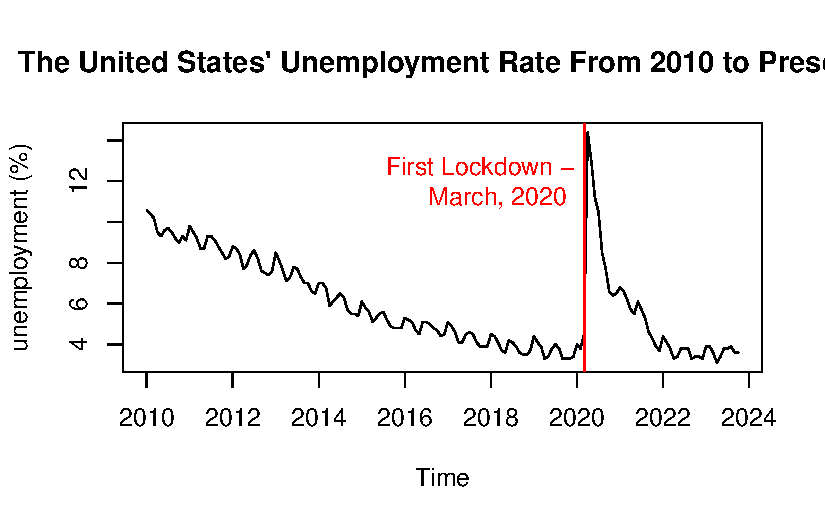
\includegraphics{Final_Project_files/figure-pdf/unnamed-chunk-1-1.pdf}

A closer look at the Pandemic:

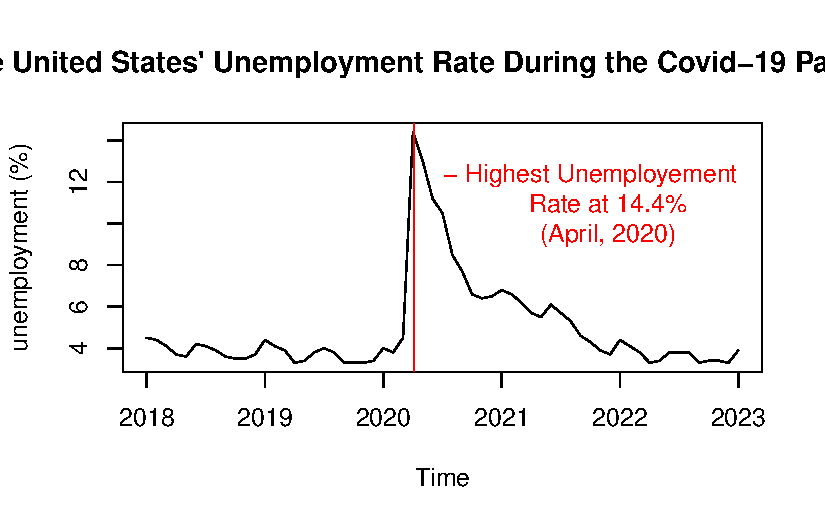
\includegraphics{Final_Project_files/figure-pdf/unnamed-chunk-2-1.pdf}

\hypertarget{training-and-testing-sets}{%
\subsection{Training and Testing Sets}\label{training-and-testing-sets}}

I will be using the years 2010-2018 for the training set and will leave
the year 2019 as the testing set for validation of forecasts.

\hypertarget{analyzing-time-series-plot-of-training-set}{%
\subsection{Analyzing Time Series Plot of Training
Set}\label{analyzing-time-series-plot-of-training-set}}

Below is the time series plot of the training set or data from
01-01-2010 to 12-01-2018:

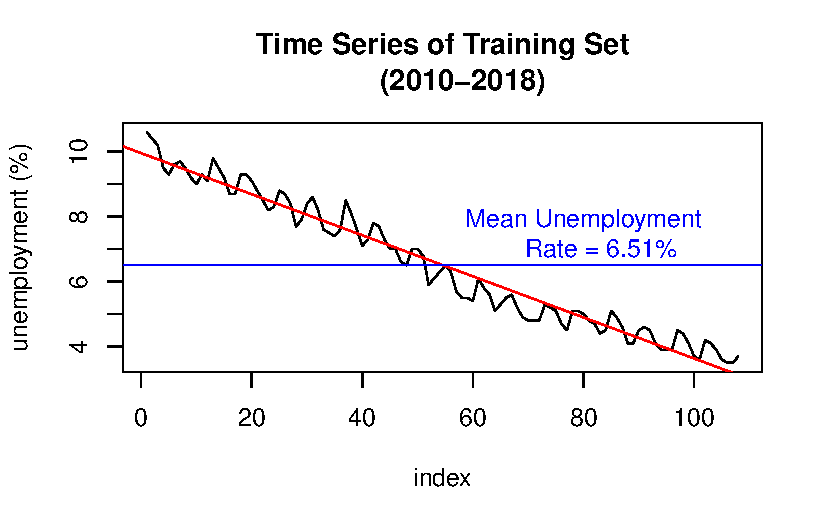
\includegraphics{Final_Project_files/figure-pdf/unnamed-chunk-4-1.pdf}

The plot shows a clear negative trend, as well as seasonality that
follows a period of 12 months. There also appears to be a slight change
in variance over time.

\hypertarget{transformation}{%
\subsection{Transformation}\label{transformation}}

Taking a look at a histogram of the data will give more information on
if the data should be transformed after seeing that there is non
constant variance.

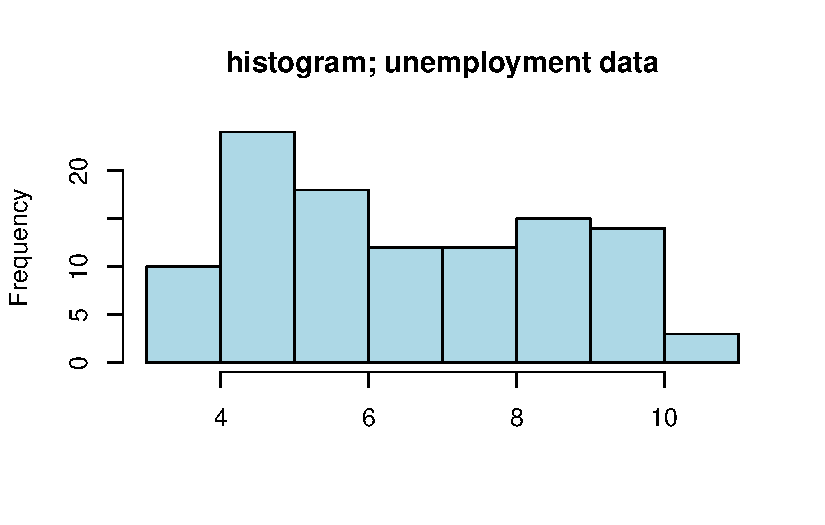
\includegraphics{Final_Project_files/figure-pdf/unnamed-chunk-5-1.pdf}

The histogram is not normal, so I will check a Box-Cox transformation.

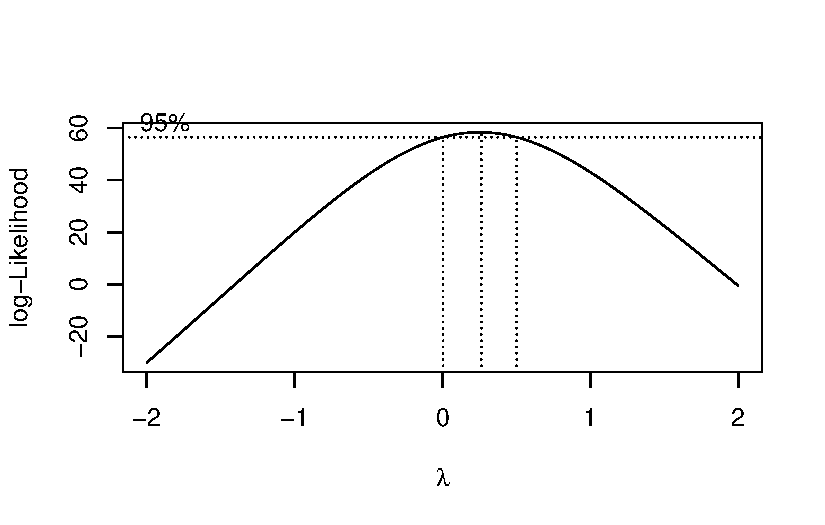
\includegraphics{Final_Project_files/figure-pdf/unnamed-chunk-6-1.pdf}

\begin{verbatim}
[1] 0.2626263
\end{verbatim}

The optimal value of lambda is 0.2626263, so I will use this value to
transform the data with the following transformation:

\[
X = Original Data
\] \[
Y = Transformed\space Data
\]

\[
Y = (X^\lambda - 1)/\lambda
\] Thus: \[
Transformed \space Data = ({Original \space Data}^{0.2626263} - 1)/0.2626263
\]

Taking a look at the time series plot of the Box-Cox transformed data:

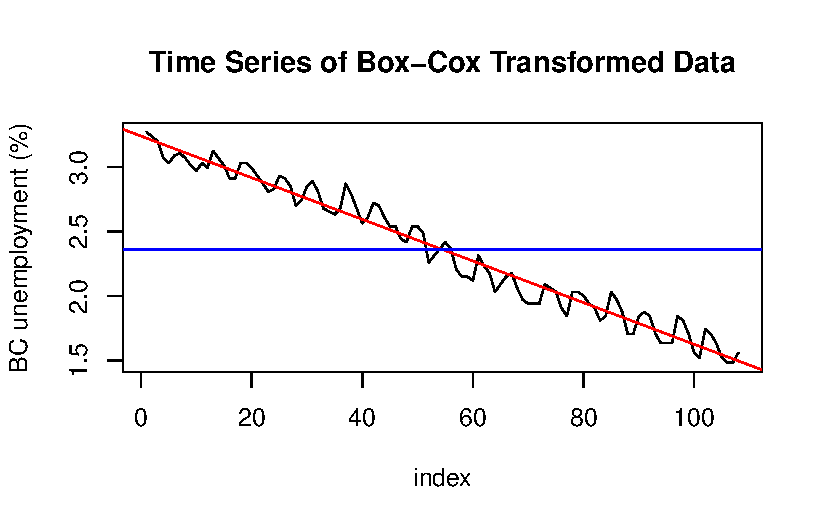
\includegraphics{Final_Project_files/figure-pdf/unnamed-chunk-7-1.pdf}

The variance appears more stable. I will also look at the histogram of
the transformed data:

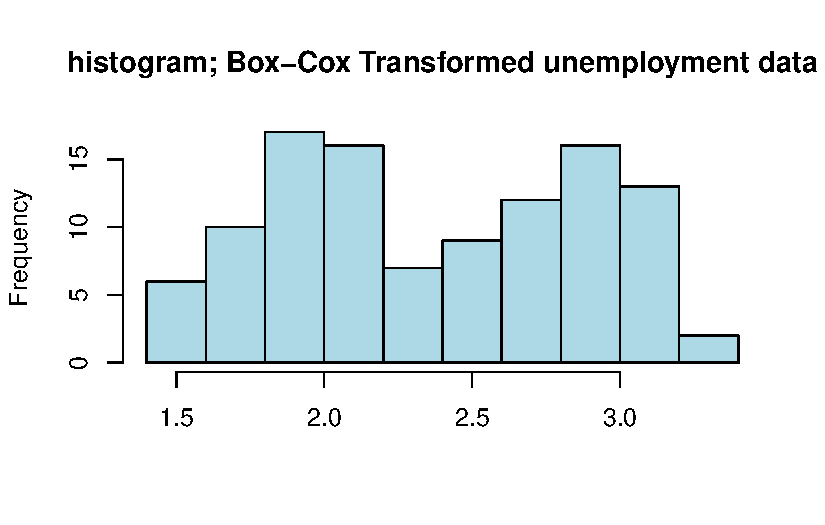
\includegraphics{Final_Project_files/figure-pdf/unnamed-chunk-8-1.pdf}

The histogram of the transformed data is not more normal than the
original data, however the variance has decreased from 4.084399 to
0.2274075 so I will keep the Box-Cox transformation.

\hypertarget{differencing}{%
\subsection{Differencing}\label{differencing}}

I will examine the Decomposition of the transformed data to determine
the neccessity for differencing.

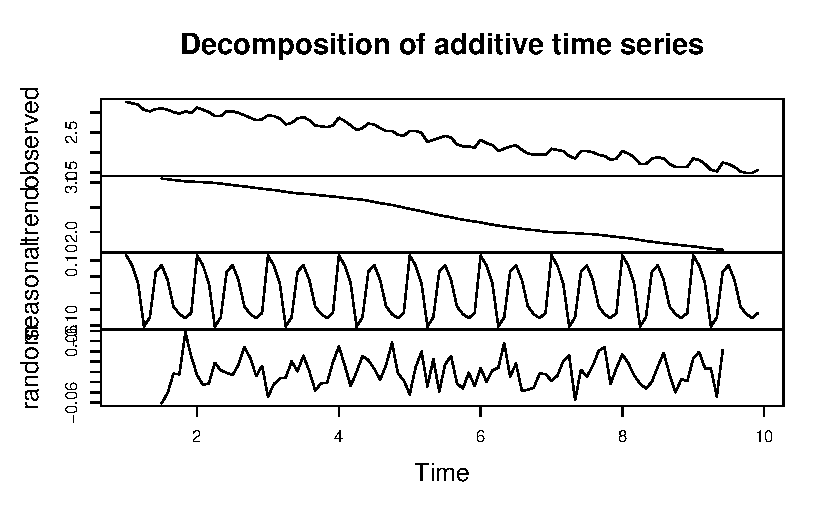
\includegraphics{Final_Project_files/figure-pdf/unnamed-chunk-9-1.pdf}

There is a clear trend and seasonality shown in the decomposition.

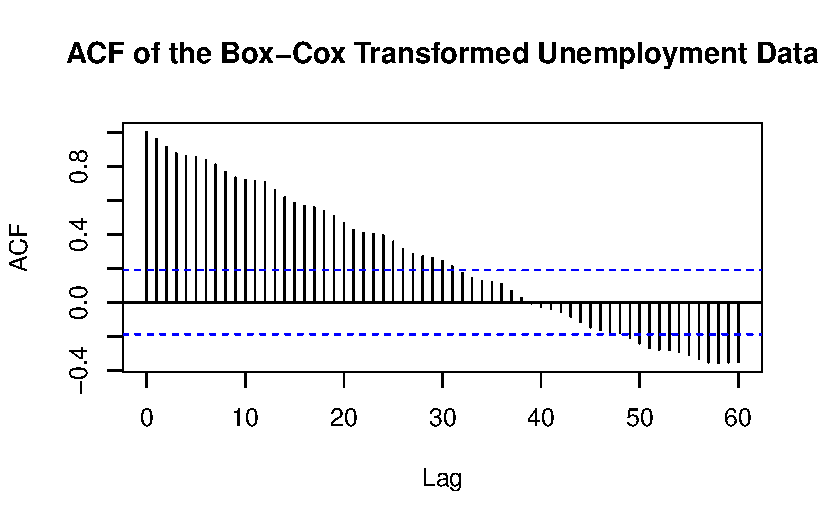
\includegraphics{Final_Project_files/figure-pdf/unnamed-chunk-10-1.pdf}

The slow decay seen in the ACF plot of the transformed data indicates
non-stationarity and there is also visible seasonality. I will begin by
differencing at lag 1 to account for the trend in the time series.

\hypertarget{differencing-at-lag-1}{%
\subsubsection{Differencing at Lag 1}\label{differencing-at-lag-1}}

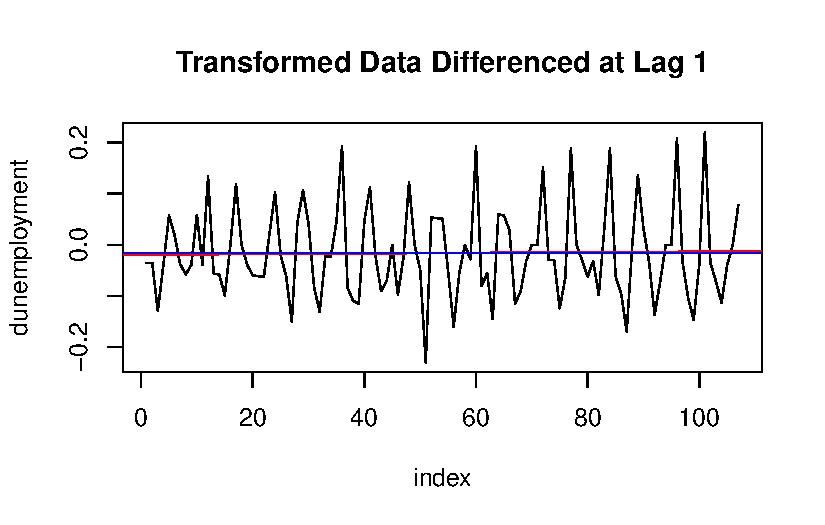
\includegraphics{Final_Project_files/figure-pdf/unnamed-chunk-11-1.pdf}

The time series plot of the transformed data differenced at lag 1 shows
constant mean and variance with no trend. I will also look at the ACF
plot to check for seasonality.

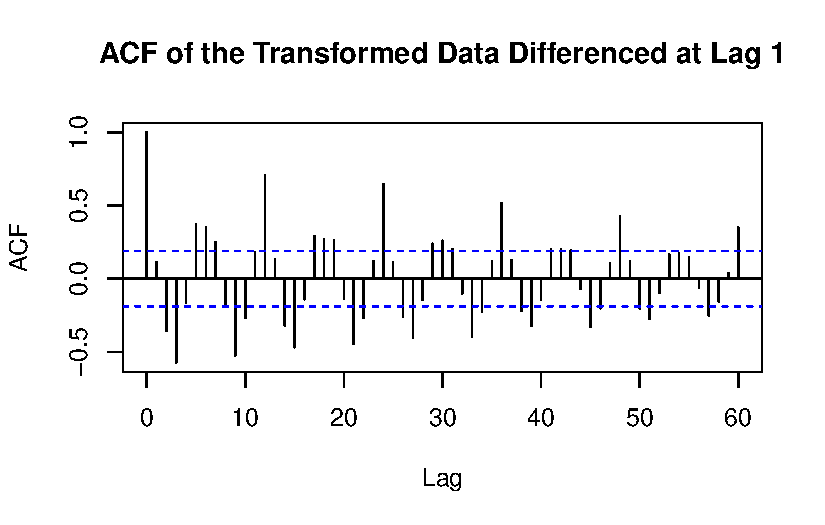
\includegraphics{Final_Project_files/figure-pdf/unnamed-chunk-12-1.pdf}

The ACF plot indicates the data is still not stationary, so I will
difference at lag 12 to account for the seasonality in the data.

\hypertarget{differencing-at-lag-12}{%
\subsubsection{Differencing at Lag 12}\label{differencing-at-lag-12}}

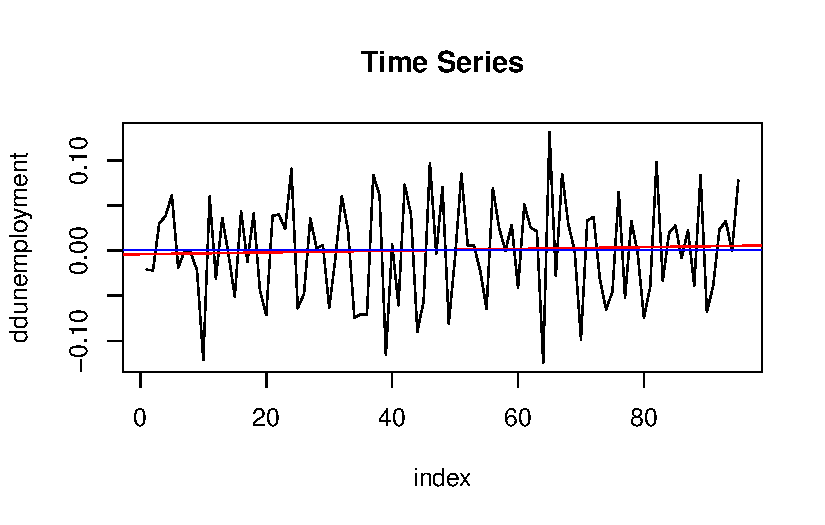
\includegraphics{Final_Project_files/figure-pdf/unnamed-chunk-13-1.pdf}

The time series plot of the transformed data differenced at lag 12 shows
constant mean and variance with no trend. I will also look at the ACF
plot to check for stationarity.

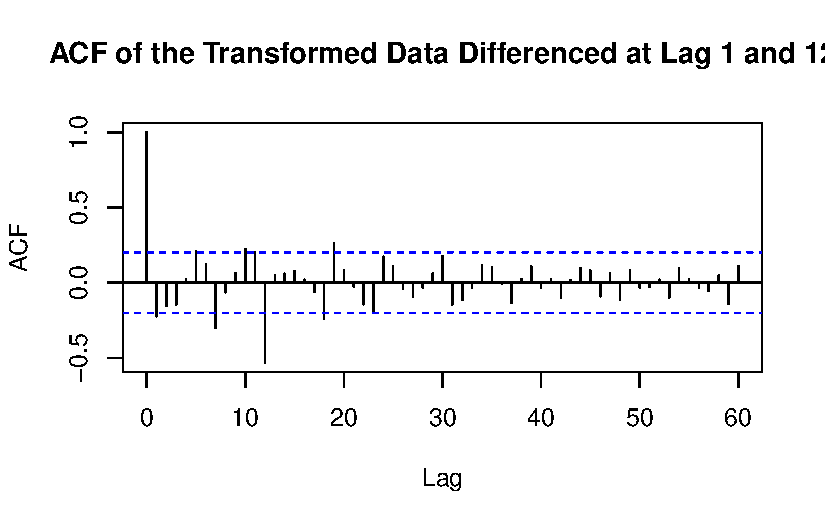
\includegraphics{Final_Project_files/figure-pdf/unnamed-chunk-14-1.pdf}

ACF decay corresponds to a stationary process.

\hypertarget{comparing-differenced-data}{%
\subsubsection{Comparing Differenced
Data}\label{comparing-differenced-data}}

I will take a look at the histograms one more time to compare the
normality of the transformed data and its differences.

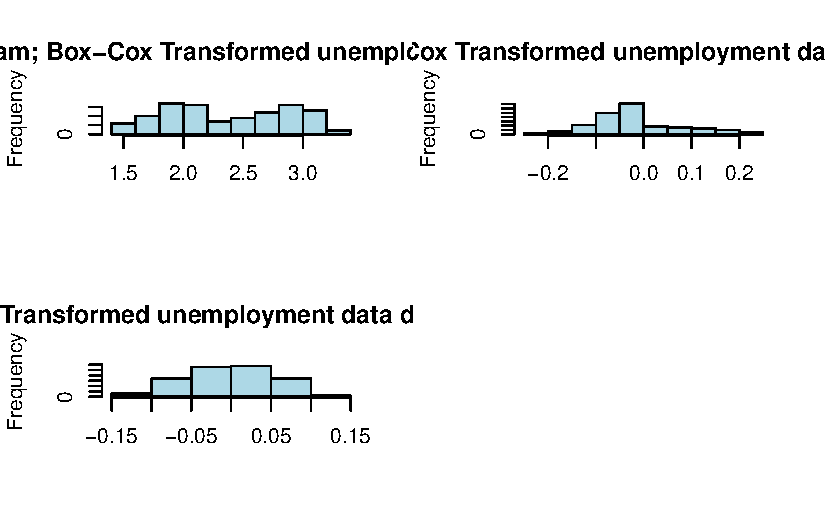
\includegraphics{Final_Project_files/figure-pdf/unnamed-chunk-15-1.pdf}

The Box-Cox transformed data differenced at lag 1 and 12 appears to be
more normally distributed than the others, as well as having decreased
variance, therefore I will continue with this data to identify the
preliminary models.

\hypertarget{identifying-preliminary-models}{%
\subsection{Identifying Preliminary
Models}\label{identifying-preliminary-models}}

To identify the candidate models, I will look at the ACF and PACF plots
of the transformed data differenced at Lags 1 and 12.

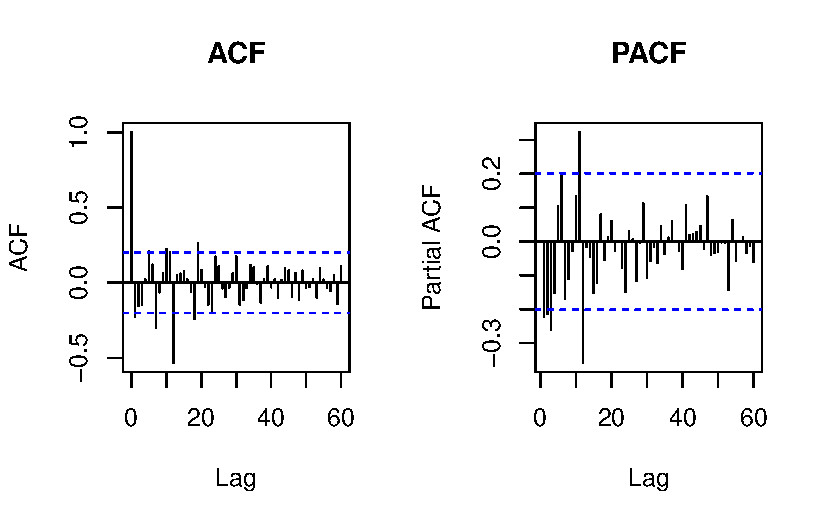
\includegraphics{Final_Project_files/figure-pdf/unnamed-chunk-16-1.pdf}

\begin{itemize}
\item
  Frist considerations:

  \begin{itemize}
  \item
    The ACF plot shows large spikes at lags 1, 7, and 12. Some SMA
    models to consider are:

    \begin{itemize}
    \item
      SARIMA(0,1,1)(0,1,1) s=12
    \item
      SARIMA(0,1,7)(0,1,1) s=12
    \end{itemize}
  \item
    I am also considering MA(12).
  \end{itemize}
\item
  Second considerations

  \begin{itemize}
  \item
    I am also keeping in mind that the ACF could be oscillating, which
    could suggest an AR or SAR model:
  \item
    The PACF plot shows large coefficients at lags 1, 2, 3, 11, and 12.
    An SAR model to try:

    \begin{itemize}
    \tightlist
    \item
      SARIMA(1,1,0)(1,1,0) s=12
    \end{itemize}
  \item
    I am also considering AR(12).
  \end{itemize}
\end{itemize}

\hypertarget{identifying-coefficients-and-model-summaries}{%
\subsubsection{Identifying Coefficients and Model
Summaries}\label{identifying-coefficients-and-model-summaries}}

\hypertarget{sarima011011-s12}{%
\paragraph{SARIMA(0,1,1)(0,1,1) s=12:}\label{sarima011011-s12}}

I will begin with the first candidate model: SARIMA(0,1,1)(0,1,1) s=12.
Below is a summary of the fitted model.

\begin{verbatim}
Registered S3 method overwritten by 'quantmod':
  method            from
  as.zoo.data.frame zoo 
\end{verbatim}

\begin{verbatim}

Call:
arima(x = bc_unemployment, order = c(0, 1, 1), seasonal = list(order = c(0, 
    1, 1), period = 12), method = "ML")

Coefficients:
          ma1     sma1
      -0.4433  -0.8196
s.e.   0.1288   0.1655

sigma^2 estimated as 0.001568:  log likelihood = 165.33,  aic = -324.65

Training set error measures:
                       ME      RMSE       MAE         MPE     MAPE      MASE
Training set -0.000581133 0.0371597 0.0283185 -0.02039254 1.311623 0.3975893
                   ACF1
Training set 0.09180784
\end{verbatim}

Both coefficients are within (-1,1) indicating the model is invertible.
I will note that the AICc value is -324.65.

\hypertarget{sarima017011-s12}{%
\paragraph{SARIMA(0,1,7)(0,1,1) s=12}\label{sarima017011-s12}}

Second, I have the candidate model: SARIMA(0,1,7)(0,1,1) s=12. Below is
a summary of the fitted model.

\begin{verbatim}

Call:
arima(x = bc_unemployment, order = c(0, 1, 7), seasonal = list(order = c(0, 
    1, 1), period = 12), method = "ML")

Coefficients:
          ma1      ma2      ma3      ma4     ma5     ma6      ma7     sma1
      -0.4058  -0.0748  -0.1606  -0.0814  0.2641  0.2601  -0.1529  -0.9998
s.e.   0.1051   0.1135   0.1018   0.1211  0.1005  0.1230   0.1083   0.2879

sigma^2 estimated as 0.001146:  log likelihood = 172.75,  aic = -327.5

Training set error measures:
                        ME       RMSE        MAE         MPE     MAPE      MASE
Training set -0.0003788741 0.03177519 0.02361649 -0.01123808 1.092566 0.3315735
                    ACF1
Training set 0.006856686
\end{verbatim}

Using the coefficient 95\% confidence intervals, I see that 0 lies
within the confidence intervals at coefficients ma2, ma3, ma4, and ma7.
Fixing for this, we then have the following summary.

\begin{verbatim}

Call:
arima(x = bc_unemployment, order = c(0, 1, 7), seasonal = list(order = c(0, 
    1, 0), period = 12), fixed = c(NA, 0, 0, 0, NA, NA, 0), method = "ML")

Coefficients:
          ma1  ma2  ma3  ma4     ma5     ma6  ma7
      -0.3912    0    0    0  0.3124  0.4353    0
s.e.   0.1579    0    0    0  0.1168  0.2030    0

sigma^2 estimated as 0.002201:  log likelihood = 151.7,  aic = -295.39

Training set error measures:
                       ME       RMSE        MAE        MPE     MAPE      MASE
Training set 0.0003164417 0.04401965 0.03226212 0.02220789 1.501236 0.4529574
                   ACF1
Training set -0.0134093
\end{verbatim}

This model has an AICc of -295.39, however I need to check that the
model is invertible. Below is a visualization of the roots (red) of the
MA polynomial.

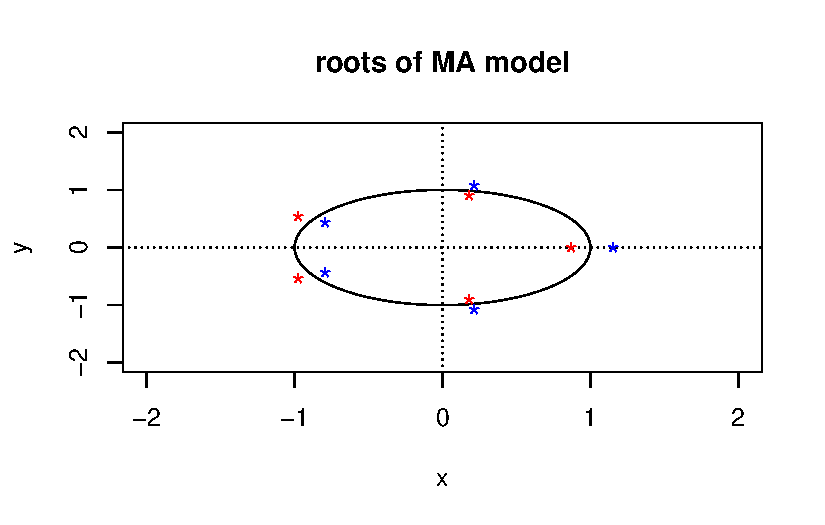
\includegraphics{Final_Project_files/figure-pdf/unnamed-chunk-20-1.pdf}

Since not all roots of the MA polynomial lie outside the unit circle,
the model is not invertible. The SARIMA(0,1,1)(0,1,1) s=12 remains as
the candidate for now.

\hypertarget{ma12}{%
\paragraph{MA(12)}\label{ma12}}

Next, I have the summary of the fitted MA(12) model.

\begin{verbatim}

Call:
arima(x = bc_unemployment, order = c(0, 1, 12), seasonal = list(order = c(0, 
    1, 0), period = 12), method = "ML")

Coefficients:
          ma1      ma2      ma3     ma4     ma5     ma6      ma7     ma8
      -0.3204  -0.0557  -0.2956  0.0568  0.1955  0.0822  -0.1458  0.0071
s.e.   0.1420   0.1444   0.1297  0.1324  0.1471  0.1428   0.1282  0.1442
          ma9    ma10     ma11     ma12
      -0.0863  0.2991  -0.0090  -0.7278
s.e.   0.1493  0.1315   0.1888   0.1591

sigma^2 estimated as 0.00132:  log likelihood = 171.51,  aic = -317.02

Training set error measures:
                       ME       RMSE        MAE        MPE     MAPE      MASE
Training set -0.000618592 0.03408784 0.02563461 -0.0111135 1.186016 0.3599077
                    ACF1
Training set -0.09433029
\end{verbatim}

Using the coefficient 95\% confidence intervals, I see that 0 lies
within the confidence intervals at coefficients ma2, ma4, ma5, ma6, ma7,
ma8, ma9, and ma11. Fixing for this, we then have the following summary.

\begin{verbatim}

Call:
arima(x = bc_unemployment, order = c(0, 1, 12), seasonal = list(order = c(0, 
    1, 0), period = 12), fixed = c(NA, 0, NA, 0, 0, 0, 0, 0, 0, NA, 0, NA), 
    method = "ML")

Coefficients:
          ma1  ma2      ma3  ma4  ma5  ma6  ma7  ma8  ma9    ma10  ma11
      -0.3020    0  -0.2158    0    0    0    0    0    0  0.2743     0
s.e.   0.0877    0   0.1137    0    0    0    0    0    0  0.1050     0
         ma12
      -0.8042
s.e.   0.1520

sigma^2 estimated as 0.001369:  log likelihood = 168.77,  aic = -327.55

Training set error measures:
                        ME       RMSE        MAE         MPE     MAPE      MASE
Training set -0.0008435405 0.03472159 0.02576233 -0.02913239 1.184669 0.3617009
                   ACF1
Training set -0.0923251
\end{verbatim}

There is now a 0 within the confidence interval for the ma3 coefficient.
So the final model summary for the MA(12) model is below.

\begin{verbatim}

Call:
arima(x = bc_unemployment, order = c(0, 1, 12), seasonal = list(order = c(0, 
    1, 0), period = 12), fixed = c(NA, 0, 0, 0, 0, 0, 0, 0, 0, NA, 0, NA), method = "ML")

Coefficients:
          ma1  ma2  ma3  ma4  ma5  ma6  ma7  ma8  ma9    ma10  ma11     ma12
      -0.3457    0    0    0    0    0    0    0    0  0.3354     0  -0.9446
s.e.   0.1182    0    0    0    0    0    0    0    0  0.1425     0   0.1516

sigma^2 estimated as 0.001235:  log likelihood = 167.21,  aic = -326.42

Training set error measures:
                        ME       RMSE        MAE         MPE     MAPE      MASE
Training set -0.0006159509 0.03297398 0.02492804 -0.01655869 1.144232 0.3499876
                  ACF1
Training set -0.112986
\end{verbatim}

This model has an AICc value of -326.42, however I need to check that
the model is invertible. Below is a visualization of the roots (red) of
the MA polynomial.

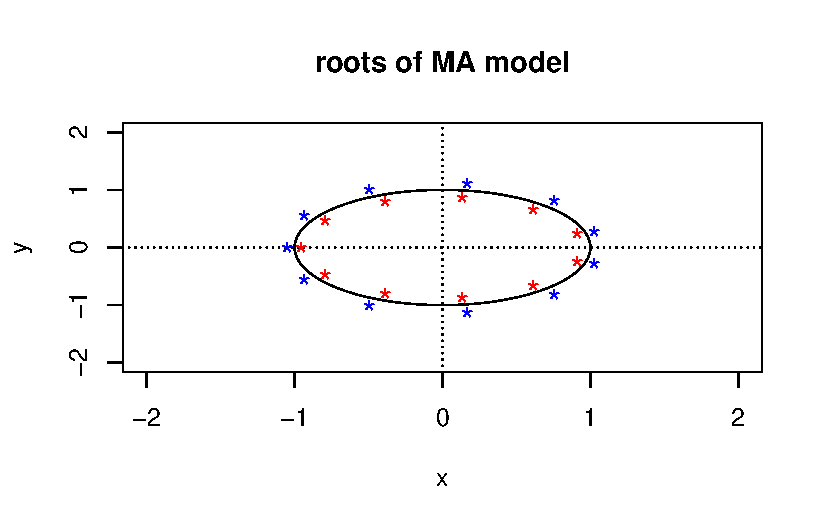
\includegraphics{Final_Project_files/figure-pdf/unnamed-chunk-24-1.pdf}

Since not all roots of the MA polynomial lie outside the unit circle,
the model is not invertible. The SARIMA(0,1,1)(0,1,1) s=12 remains as
the candidate for now.

\hypertarget{sarima110110-s12}{%
\paragraph{SARIMA(1,1,0)(1,1,0) s=12}\label{sarima110110-s12}}

Due to the possible decay I saw in the ACF plot of the differenced data,
I am also considering the SARIMA(1,1,0)(1,1,0) s=12 model and below is a
summary of the fitted model.

\begin{verbatim}

Call:
arima(x = bc_unemployment, order = c(1, 1, 0), seasonal = list(order = c(1, 
    1, 0), period = 12), method = "ML")

Coefficients:
          ar1     sar1
      -0.2172  -0.5605
s.e.   0.1005   0.0818

sigma^2 estimated as 0.001904:  log likelihood = 160.45,  aic = -314.9

Training set error measures:
                       ME       RMSE        MAE        MPE     MAPE      MASE
Training set 0.0003003032 0.04093835 0.03163286 0.02096746 1.469947 0.4441226
                    ACF1
Training set -0.02973299
\end{verbatim}

Both coefficients are within (-1,1), indicating the model is stationary.
I will note that the AICc value is -314.9

\hypertarget{ar12}{%
\paragraph{AR(12)}\label{ar12}}

Next I have the summary of the fitted AR(12) model.

\begin{verbatim}

Call:
arima(x = bc_unemployment, order = c(12, 1, 0), seasonal = list(order = c(0, 
    1, 0), period = 12), method = "ML")

Coefficients:
          ar1      ar2      ar3      ar4      ar5     ar6      ar7      ar8
      -0.2831  -0.1303  -0.1247  -0.0834  -0.0196  0.1251  -0.0998  -0.0368
s.e.   0.0946   0.0970   0.0966   0.0989   0.1001  0.1032   0.1001   0.0997
         ar9    ar10    ar11     ar12
      0.0430  0.1708  0.1729  -0.3894
s.e.  0.1007  0.1050  0.1049   0.0994

sigma^2 estimated as 0.001625:  log likelihood = 168.11,  aic = -310.22

Training set error measures:
                       ME       RMSE        MAE        MPE     MAPE      MASE
Training set 0.0002981154 0.03782493 0.02797456 0.02067937 1.293941 0.3927603
                   ACF1
Training set -0.0084127
\end{verbatim}

Using the coefficient 95\% confidence intervals, I see that 0 lies
within the confidence intervals at coefficients ar2, ar3, ar4, ar5, ar6,
ar7, ar8, ar9, ar10, and ar11. Fixing for this, we then have the
following summary.

\begin{verbatim}

Call:
arima(x = bc_unemployment, order = c(12, 1, 0), seasonal = list(order = c(0, 
    1, 0), period = 12), fixed = c(NA, 0, 0, 0, 0, 0, 0, 0, 0, 0, 0, NA), method = "ML")

Coefficients:
          ar1  ar2  ar3  ar4  ar5  ar6  ar7  ar8  ar9  ar10  ar11     ar12
      -0.1135    0    0    0    0    0    0    0    0     0     0  -0.5415
s.e.   0.0831    0    0    0    0    0    0    0    0     0     0   0.0834

sigma^2 estimated as 0.001965:  log likelihood = 159.1,  aic = -312.2

Training set error measures:
                       ME      RMSE        MAE        MPE     MAPE      MASE
Training set 0.0003152606 0.0415873 0.03190487 0.02248603 1.479125 0.4479416
                   ACF1
Training set -0.1071929
\end{verbatim}

There is now a 0 within the confidence interval for the ar1 coefficient.
So the final model summary for the MA(12) model is below.

\begin{verbatim}

Call:
arima(x = bc_unemployment, order = c(12, 1, 0), seasonal = list(order = c(0, 
    1, 0), period = 12), fixed = c(0, 0, 0, 0, 0, 0, 0, 0, 0, 0, 0, NA), method = "ML")

Coefficients:
      ar1  ar2  ar3  ar4  ar5  ar6  ar7  ar8  ar9  ar10  ar11     ar12
        0    0    0    0    0    0    0    0    0     0     0  -0.5637
s.e.    0    0    0    0    0    0    0    0    0     0     0   0.0817

sigma^2 estimated as 0.001997:  log likelihood = 158.17,  aic = -312.34

Training set error measures:
                       ME       RMSE        MAE        MPE     MAPE      MASE
Training set 0.0003058091 0.04192702 0.03239767 0.02188477 1.499944 0.4548605
                   ACF1
Training set -0.2133004
\end{verbatim}

The only coefficient left is for ar12 and it is within (-1,1) thus the
model is stationary. I will note that the AICc value is -312.34

\hypertarget{comparing-models}{%
\subsection{Comparing Models}\label{comparing-models}}

The candidate models which are both stationary and invertible have the
following AICc values:

\begin{itemize}
\item
  SARIMA(0,1,1)(0,1,1) s=12

  \begin{itemize}
  \tightlist
  \item
    AICc = -324.65
  \end{itemize}
\item
  SARIMA(1,1,0)(1,1,0) s=12

  \begin{itemize}
  \tightlist
  \item
    AICc = -314.9
  \end{itemize}
\item
  AR(12)

  \begin{itemize}
  \tightlist
  \item
    AICc = -312.34
  \end{itemize}
\end{itemize}

Based on this information, I will continue with the SARIMA(0,1,1)(0,1,1)
s=12 model for diagnostic checking since it has the lowest AICc value of
-324.65.

\hypertarget{chosen-model-sarima011011-s12}{%
\paragraph{Chosen Model: SARIMA(0,1,1)(0,1,1)
s=12}\label{chosen-model-sarima011011-s12}}

\[
(1+0.4433B)(1+0.8196B^{12})(1-B)(1-B^{12}){X_t} = {Z_t} \space \space
\] \[
Where \space {Z_t} \sim WN(0,{\sigma_Z}^2)
\]

\hypertarget{residual-analysis-and-diagnostic-checking}{%
\subsection{Residual Analysis and Diagnostic
Checking}\label{residual-analysis-and-diagnostic-checking}}

\hypertarget{visualizing-residuals}{%
\subsubsection{Visualizing Residuals}\label{visualizing-residuals}}

Below are visualizations of the SARIMA(0,1,1)(0,1,1) s=12 model's
residuals to check that they are Gaussian and follow a White Noise
pattern.

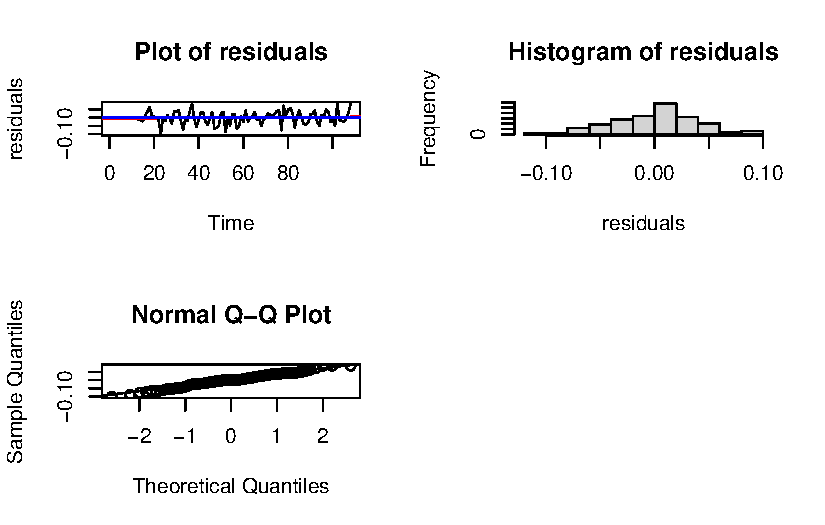
\includegraphics{Final_Project_files/figure-pdf/unnamed-chunk-30-1.pdf}

The plotted residuals do resemble white noise and the trend and mean
appear to coincide at about 0. The residuals distribution is
approximately normal centered at 0. In the qq plot, the dots do follow
close to the line.

\hypertarget{acf-and-pacf-plots-of-residuals}{%
\subsubsection{ACF and PACF Plots of
Residuals}\label{acf-and-pacf-plots-of-residuals}}

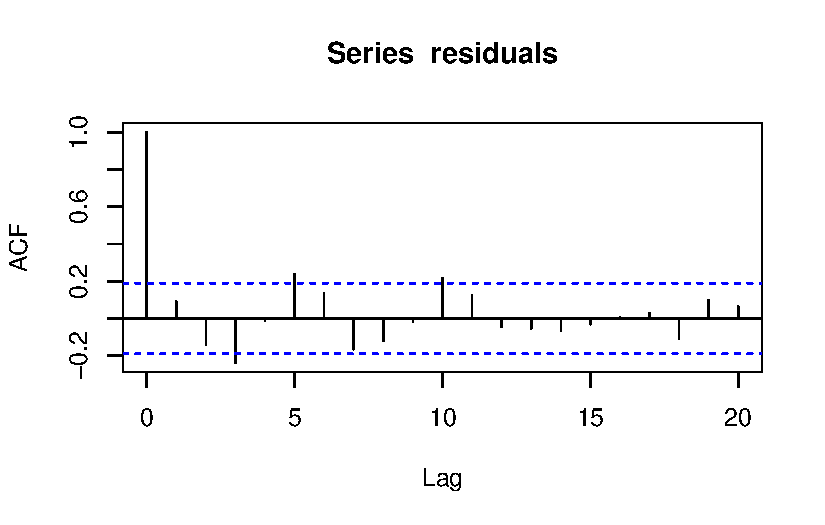
\includegraphics{Final_Project_files/figure-pdf/unnamed-chunk-31-1.pdf}

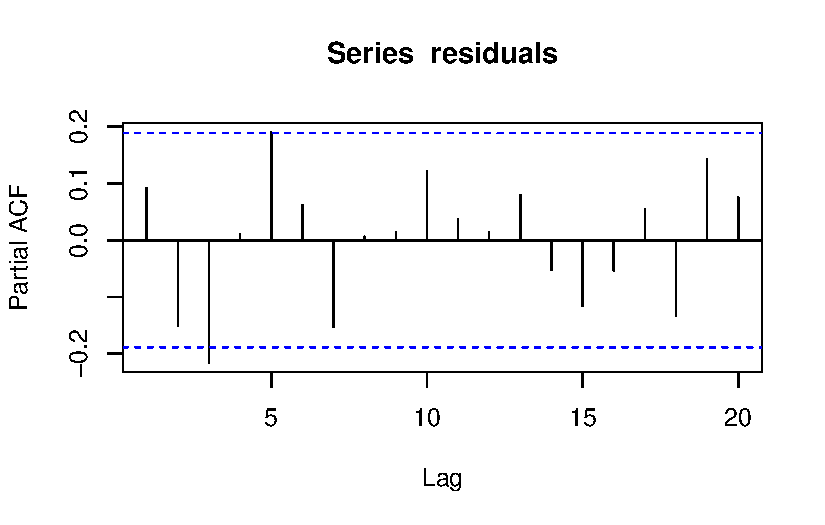
\includegraphics{Final_Project_files/figure-pdf/unnamed-chunk-31-2.pdf}

I want all coefficients at lags \textgreater{} 1 to be within the
confidence intervals. There are a few lags that have coefficients
slightly outside the confidence interval, however they are not large and
I am happy with the normality of the residuals.

\hypertarget{shapiro-wilk-test-of-normality}{%
\subsubsection{Shapiro-Wilk Test of
Normality}\label{shapiro-wilk-test-of-normality}}

I will also be using the Shapiro-Wilk Test to check that the residuals
are normally distributed.

\begin{verbatim}

    Shapiro-Wilk normality test

data:  residuals
W = 0.98708, p-value = 0.387
\end{verbatim}

The p-value is 0.387, which is larger than 0.05, so I fail to reject the
normality hypothesis of the residuals.

\hypertarget{portmanteau-statistics}{%
\subsubsection{Portmanteau Statistics}\label{portmanteau-statistics}}

Another part of diagnostic checking are the Portmanteau Statistics,
checking for p-values \textless{} 0.05.

Both the Box-Pierce and Ljung-Box Tests are to test for linear
dependence of the residuals. Since there are 108 observations in the
training set, lag = 10, and since I have 2 estimated coefficients (ma1
and sma1) the fitdf = 2 for these two tests.

The McLeod-Li Test is to test if the residuals are correlated and uses
the same lag = 10 and fitdf = 0.

\hypertarget{box-pierce-test}{%
\paragraph{Box-Pierce Test}\label{box-pierce-test}}

\begin{verbatim}

    Box-Pierce test

data:  residuals
X-squared = 26.763, df = 8, p-value = 0.0007766
\end{verbatim}

\hypertarget{ljung-box-test}{%
\paragraph{Ljung-Box Test}\label{ljung-box-test}}

\begin{verbatim}

    Box-Ljung test

data:  residuals
X-squared = 28.764, df = 8, p-value = 0.0003488
\end{verbatim}

\hypertarget{mcleod-li-test}{%
\paragraph{McLeod-Li Test}\label{mcleod-li-test}}

\begin{verbatim}

    Box-Ljung test

data:  residuals^2
X-squared = 8.5701, df = 10, p-value = 0.5733
\end{verbatim}

P-values for both the Box-Pierce and Ljung-Box Tests are below 0.05,
meaning I reject the hypothesis that the residuals are linearly
independent.

The p-value for the McLeod-Li Test is greater than 0.05, meaning I fail
to reject the hypothesis that the residuals are uncorrelated.

I note that the fitted model's residuals do not pass the Box-Pierce and
Ljung-Box Tests, however I will continue to forecasting based on the
residuals passing all other diagnostic checks.

\hypertarget{forecasting}{%
\subsection{Forecasting}\label{forecasting}}

\hypertarget{forecasting-on-transformed-data}{%
\subsubsection{Forecasting on Transformed
Data}\label{forecasting-on-transformed-data}}

Below are the plotted forecast values on the Box-Cox transformed data

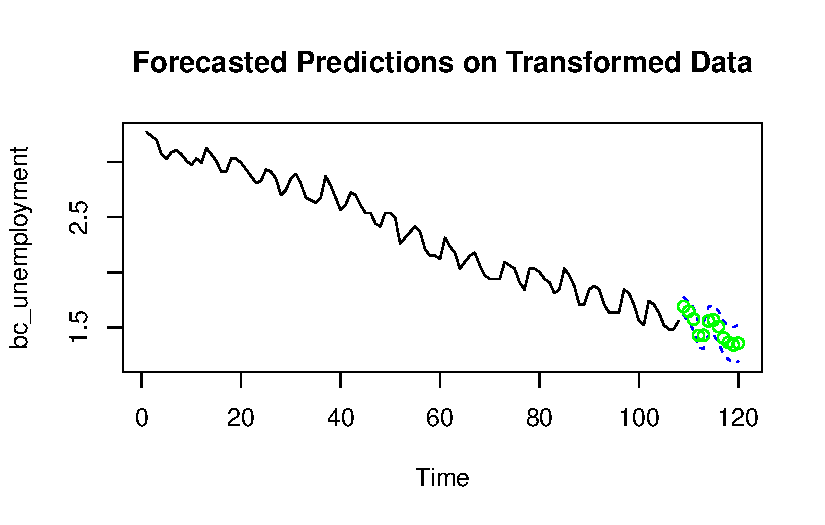
\includegraphics{Final_Project_files/figure-pdf/unnamed-chunk-36-1.pdf}

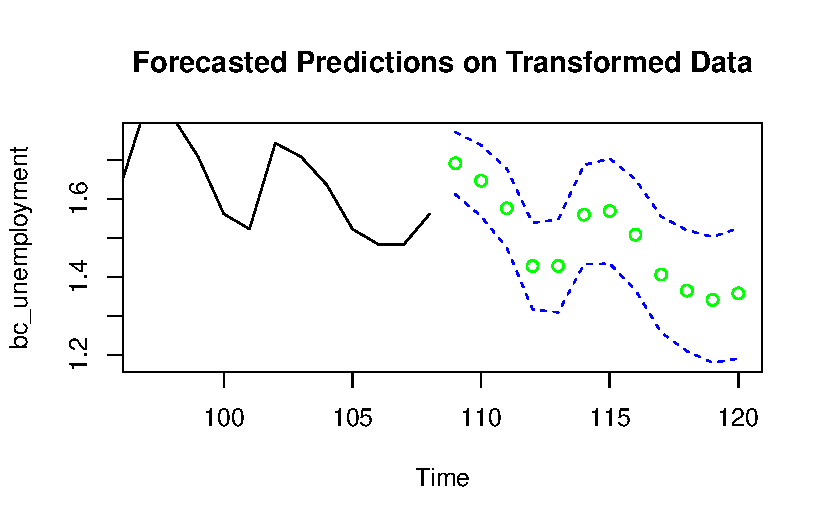
\includegraphics{Final_Project_files/figure-pdf/unnamed-chunk-36-2.pdf}

\hypertarget{forecasting-on-original-data}{%
\subsubsection{Forecasting on Original
Data}\label{forecasting-on-original-data}}

After transforming the predicted values back to the original data
values, below are the plotted forecast values on the original
unemployment data as well as the test set values.

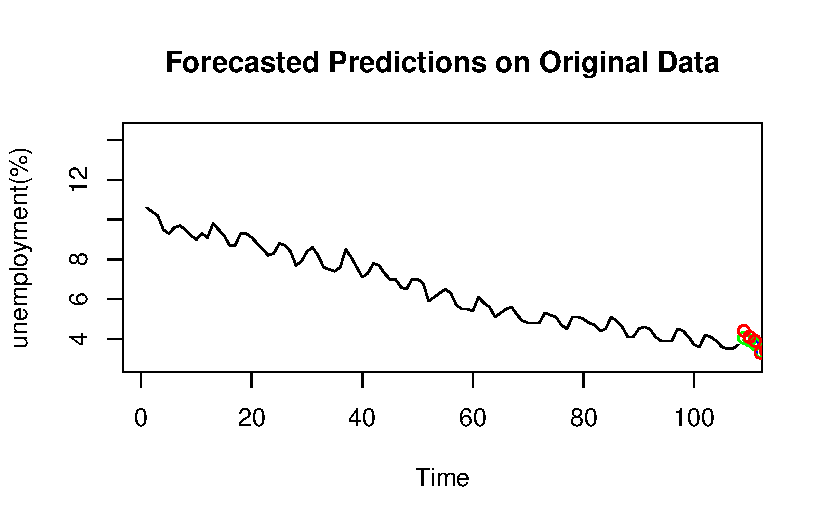
\includegraphics{Final_Project_files/figure-pdf/unnamed-chunk-37-1.pdf}

Below is a closer look at the model's predicted values (green) compared
to the observed test values (red) as well as the 95\% confidence
interval for forecast values (blue).

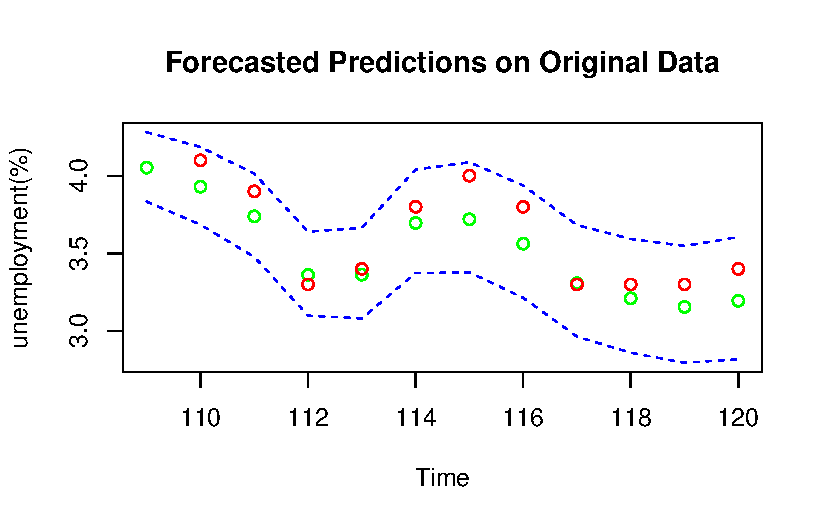
\includegraphics{Final_Project_files/figure-pdf/unnamed-chunk-38-1.pdf}

Looking to the test values (red) which all lie within the 95\%
confidence interval, I am able to validate the SARIMA(0,1,1)(0,1,1) s=12
model's ability to accurately forecast unemployment rates into the year
2019.

\hypertarget{forecasting-through-2023}{%
\subsubsection{Forecasting through
2023}\label{forecasting-through-2023}}

Below is the predicted unemployment rate time series through the years
2020-2023 as compared to the observed times series.

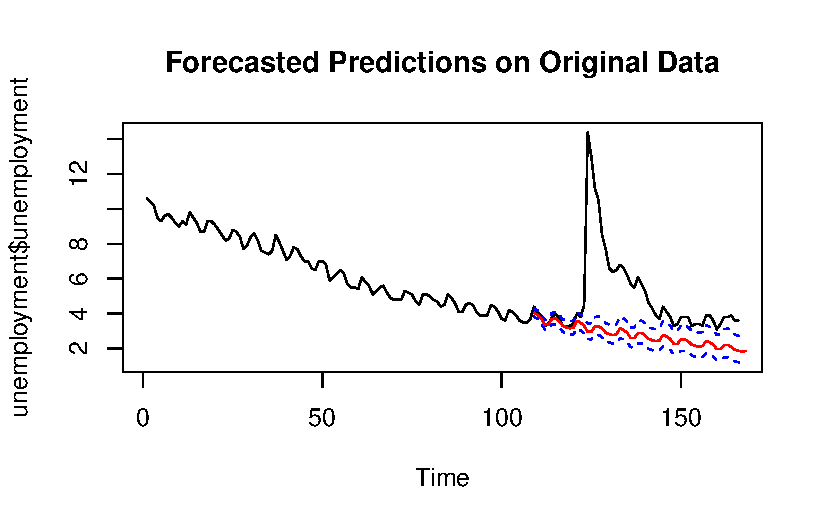
\includegraphics{Final_Project_files/figure-pdf/unnamed-chunk-39-1.pdf}

We can take a closer look at the years 2019 through October, 2023.

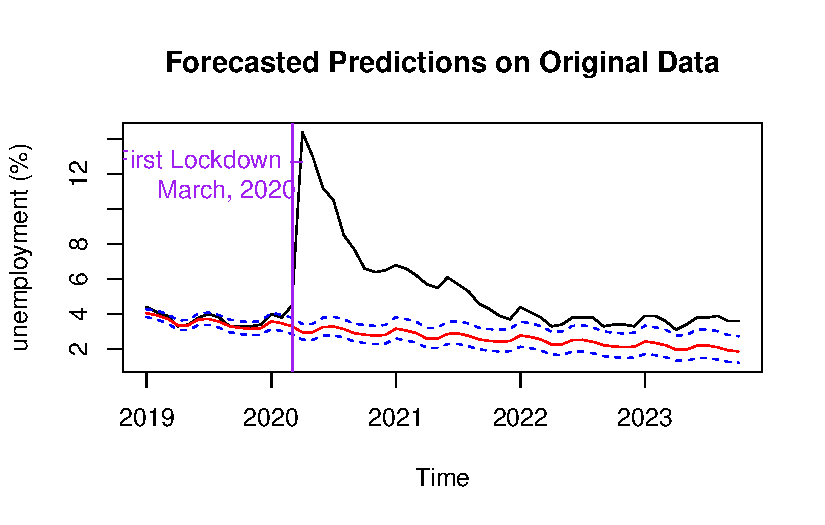
\includegraphics{Final_Project_files/figure-pdf/unnamed-chunk-40-1.pdf}

While the observed unemployment values of 2019 appear to coincide with
the prediction intervals, there is a large difference beginning in early
2020. Unemployment rates remain much higher than the predicted interval
until the end of 2021. From the beginning of 2022 and up through October
of 2023, unemployment rates are still higher than the upper side of the
prediction interval.

The predicted unemployment rate for October of 2023 based on data from
2010 to 2018 is 1.86\%, whereas the observed unemployment rate at the
beginning of October this year was 3.6\%, almost twice as high. Because
of the seasonality, the best comparison to pre-pandemic levels would be
the October prior to the start of the Pandemic. The unemployment rate at
the beginning of October, 2019 was 3.3\% so levels are still higher. It
would be interesting to compare the unemployment rate of March, 2024 to
March, 2020 to see if unemployment finally decreases to pre-pandemic
levels.

\hypertarget{conclusion}{%
\subsection{Conclusion}\label{conclusion}}

The goal of this project was to forecast unemployment rates through 2023
using data from 2010-2018 fitted to a Seasonal Autoregressive Integrated
Moving Average (SARIMA) model.

Using the SARIMA(0,1,1)(0,1,1) s=12 model:

\[
(1+0.4433B)(1+0.8196B^{12})(1-B)(1-B^{12}){X_t} = {Z_t} \space \space
\] \[
Where \space {Z_t} \sim WN(0,{\sigma_Z}^2)
\]

I hoped to compare and contrast the unemployment rates observed during
and after the Covid-19 Pandemic to the predicted values. I found there
was a large spike in the unemployment rate during the beginning months
of 2020 which decreased during the second half of the year, but did not
decrease to pre-pandemic levels until 2022, and were still slightly
higher. Based on the trend seen for the unemployment level from 2010 to
2018, the unemployment rate is predicted to be just 1.86\% in October,
and 1.85\% on December 1, 2023. These predictions are proportionally
about half of what the unemployment levels are today, meaning twice as
many Americans are out of work than what this model predicts if the
Covid-19 Pandemic had not occurred.

That being said, anomalous events have occurred throughout American
history that disrupt the trend in unemployment levels, therefore
something else could have impacted unemployment rates during this time
without the Pandemic. It is worth noting that April, 2020 did mark the
largest unemployment rate in United States' history since 1940 after the
lasting effects of the Great Depression (Amadeo, 2022). Comparing these
forecast values to the unemployment rates observed after the Covid-19
Pandemic can help national and state governments prepare for the impact
another anomalous event may have on the unemployment rate, and then
predict the amount of time it may take to reach unemployment levels
prior to the event.

I want to acknowledge Professor Raisa Feldman and Teaching Assistant
Cosmin Borsa for guiding me through this project and providing
assistance and understanding.

\hypertarget{references}{%
\subsection{References}\label{references}}

Amadeo, Kimberly. "Historical US Unemployment Rate by Year." \emph{The
Balance}, The Balance, 6 Dec.~2022,
www.thebalancemoney.com/unemployment-rate-by-year-3305506\#:\textasciitilde:text=The\%20highest\%20rate\%20of\%20U.S.,14\%25\%20from\%201931\%20to\%201940.

Duggan, Wayne. "A Short h=History of the Great Recession."
\emph{Forbes}, Forbes Magazine, 21 June 2023,
www.forbes.com/advisor/investing/great-recession/\#:\textasciitilde:text=The\%20Great\%20Recession\%20of\%202008,down\%2057\%25\%20from\%20its\%20highs.),.

"Unemployment Rate (UNRATENSA)." \emph{FRED}, 3 Nov.~2023,
fred.stlouisfed.org/series/UNRATENSA.

\hypertarget{appendix}{%
\subsection{Appendix}\label{appendix}}

The following is code for each of the visuals, model summaries, and
tests performed in this report.

\hypertarget{visualizing-unemployment-time-series-from-2010-to-present}{%
\subparagraph{Visualizing unemployment time series from 2010 to
present:}\label{visualizing-unemployment-time-series-from-2010-to-present}}

\begin{Shaded}
\begin{Highlighting}[]
\NormalTok{unemployment }\OtherTok{\textless{}{-}} \FunctionTok{read.csv}\NormalTok{(}\StringTok{"data/unemployment.csv"}\NormalTok{)}

\CommentTok{\# converting to datetime object }
\NormalTok{unemployment[[}\StringTok{\textquotesingle{}Date\textquotesingle{}}\NormalTok{]] }\OtherTok{\textless{}{-}} \FunctionTok{as.Date}\NormalTok{(unemployment[[}\DecValTok{1}\NormalTok{]],}
                                  \AttributeTok{format =}\StringTok{"\%Y{-}\%d{-}\%m"}\NormalTok{)}

\NormalTok{unemployment\_ts }\OtherTok{\textless{}{-}} \FunctionTok{ts}\NormalTok{(unemployment}\SpecialCharTok{$}\NormalTok{unemployment , }\AttributeTok{frequency =} \DecValTok{12}\NormalTok{, }\AttributeTok{start=}\FunctionTok{c}\NormalTok{(}\DecValTok{2010}\NormalTok{,}\DecValTok{1}\NormalTok{), }\AttributeTok{end =} \FunctionTok{c}\NormalTok{(}\DecValTok{2023}\NormalTok{,}\DecValTok{10}\NormalTok{))}

\CommentTok{\# visualize data from 2010 to present}
\FunctionTok{plot.ts}\NormalTok{(unemployment\_ts, }\AttributeTok{ylab =} \StringTok{"unemployment (\%)"}\NormalTok{, }\AttributeTok{main =} \StringTok{"The United States\textquotesingle{} Unemployment Rate From 2010 to Present"}\NormalTok{)}
\FunctionTok{abline}\NormalTok{(}\AttributeTok{v=}\FunctionTok{c}\NormalTok{(}\FloatTok{2020.2}\NormalTok{,}\DecValTok{3}\NormalTok{), }\AttributeTok{col =} \StringTok{"red"}\NormalTok{)}
\FunctionTok{text}\NormalTok{(}\AttributeTok{x =} \FunctionTok{c}\NormalTok{(}\FloatTok{2017.75}\NormalTok{,}\DecValTok{3}\NormalTok{), }\AttributeTok{y =} \DecValTok{12}\NormalTok{,}\StringTok{"First Lockdown {-}}
\StringTok{     March 2020"}\NormalTok{, }\AttributeTok{col =} \StringTok{"red"}\NormalTok{)}
\end{Highlighting}
\end{Shaded}

\hypertarget{zoomed-in-time-series}{%
\subparagraph{Zoomed in time series:}\label{zoomed-in-time-series}}

\begin{Shaded}
\begin{Highlighting}[]
\NormalTok{unemployment\_ts2 }\OtherTok{\textless{}{-}} \FunctionTok{ts}\NormalTok{(unemployment}\SpecialCharTok{$}\NormalTok{unemployment[}\DecValTok{97}\SpecialCharTok{:}\DecValTok{166}\NormalTok{], }\AttributeTok{frequency =} \DecValTok{12}\NormalTok{, }\AttributeTok{start=}\FunctionTok{c}\NormalTok{(}\DecValTok{2018}\NormalTok{), }\AttributeTok{end =} \FunctionTok{c}\NormalTok{(}\DecValTok{2023}\NormalTok{))}

\CommentTok{\# visualize data from 2010 to present}
\FunctionTok{plot.ts}\NormalTok{(unemployment\_ts2, }\AttributeTok{ylab =} \StringTok{"unemployment (\%)"}\NormalTok{, }\AttributeTok{main =} \StringTok{"The United States\textquotesingle{} Unemployment Rate During the Covid{-}19 Pandemic"}\NormalTok{)}
\FunctionTok{abline}\NormalTok{(}\AttributeTok{v=}\FunctionTok{c}\NormalTok{(}\DecValTok{4}\NormalTok{,}\FloatTok{2020.26}\NormalTok{), }\AttributeTok{col =} \StringTok{"red"}\NormalTok{)}
\FunctionTok{text}\NormalTok{(}\AttributeTok{x =} \FunctionTok{c}\NormalTok{(}\DecValTok{3}\NormalTok{,}\FloatTok{2021.75}\NormalTok{), }\AttributeTok{y =} \DecValTok{11}\NormalTok{,}\StringTok{"{-} Highest Unemployement}
\StringTok{     Rate at 14.4\%}
\StringTok{     (April, 2020)"}\NormalTok{, }\AttributeTok{col =} \StringTok{"red"}\NormalTok{)}
\end{Highlighting}
\end{Shaded}

\hypertarget{training-and-testing-sets-1}{%
\subparagraph{Training and testing
sets:}\label{training-and-testing-sets-1}}

\begin{Shaded}
\begin{Highlighting}[]
\NormalTok{train }\OtherTok{\textless{}{-}}\NormalTok{ unemployment\_ts[}\FunctionTok{c}\NormalTok{(}\DecValTok{1}\SpecialCharTok{:}\DecValTok{108}\NormalTok{)]}
\CommentTok{\# leaving out 12 data points for testing set}
\NormalTok{test }\OtherTok{\textless{}{-}}\NormalTok{ unemployment\_ts[}\FunctionTok{c}\NormalTok{(}\DecValTok{109}\SpecialCharTok{:}\DecValTok{120}\NormalTok{)]}
\end{Highlighting}
\end{Shaded}

\hypertarget{time-series-plot-of-training-set}{%
\subparagraph{Time series plot of training
set:}\label{time-series-plot-of-training-set}}

\begin{Shaded}
\begin{Highlighting}[]
\FunctionTok{plot}\NormalTok{(}\DecValTok{1}\SpecialCharTok{:}\FunctionTok{length}\NormalTok{(train),train, }\AttributeTok{main =} \StringTok{"Time Series of Training Set}
\StringTok{     (2010{-}2018)"}\NormalTok{, }\AttributeTok{type =} \StringTok{\textquotesingle{}l\textquotesingle{}}\NormalTok{,}\AttributeTok{xlab=}\StringTok{\textquotesingle{}index\textquotesingle{}}\NormalTok{, }\AttributeTok{ylab =} \StringTok{"unemployment (\%)"}\NormalTok{)}

\NormalTok{index }\OtherTok{=} \DecValTok{1}\SpecialCharTok{:} \FunctionTok{length}\NormalTok{(train)}
\NormalTok{trend }\OtherTok{\textless{}{-}} \FunctionTok{lm}\NormalTok{(train }\SpecialCharTok{\textasciitilde{}}\NormalTok{ index)}
\FunctionTok{abline}\NormalTok{(trend, }\AttributeTok{col=}\StringTok{"red"}\NormalTok{)}
\FunctionTok{abline}\NormalTok{(}\AttributeTok{h=}\FunctionTok{mean}\NormalTok{(train) , }\AttributeTok{col=}\StringTok{\textquotesingle{}blue\textquotesingle{}}\NormalTok{)}
\FunctionTok{text}\NormalTok{(}\AttributeTok{x =} \FunctionTok{c}\NormalTok{(}\DecValTok{80}\NormalTok{), }\AttributeTok{y =} \FloatTok{7.5}\NormalTok{,}\StringTok{"Mean Unemployment}
\StringTok{     Rate = 6.51\%"}\NormalTok{, }\AttributeTok{col =} \StringTok{"blue"}\NormalTok{)}
\end{Highlighting}
\end{Shaded}

\hypertarget{histogram-of-training-data}{%
\subparagraph{Histogram of training
data:}\label{histogram-of-training-data}}

\begin{Shaded}
\begin{Highlighting}[]
\FunctionTok{hist}\NormalTok{(train, }\AttributeTok{col=}\StringTok{"light blue"}\NormalTok{, }\AttributeTok{xlab=}\StringTok{""}\NormalTok{, }\AttributeTok{main=}\StringTok{"histogram; unemployment data"}\NormalTok{)}
\end{Highlighting}
\end{Shaded}

\hypertarget{box-cox-diagram-and-lambda-value}{%
\subparagraph{Box-Cox diagram and lambda
value:}\label{box-cox-diagram-and-lambda-value}}

\begin{Shaded}
\begin{Highlighting}[]
\FunctionTok{library}\NormalTok{(MASS)}
\NormalTok{bcTransform }\OtherTok{\textless{}{-}} \FunctionTok{boxcox}\NormalTok{(train}\SpecialCharTok{\textasciitilde{}}\FunctionTok{as.numeric}\NormalTok{(}\DecValTok{1}\SpecialCharTok{:}\FunctionTok{length}\NormalTok{(train)))}
\CommentTok{\# optimal lambda}
\NormalTok{lambda }\OtherTok{\textless{}{-}}\NormalTok{ bcTransform}\SpecialCharTok{$}\NormalTok{x[}\FunctionTok{which}\NormalTok{(bcTransform}\SpecialCharTok{$}\NormalTok{y }\SpecialCharTok{==} \FunctionTok{max}\NormalTok{(bcTransform}\SpecialCharTok{$}\NormalTok{y))]}
\NormalTok{lambda}
\end{Highlighting}
\end{Shaded}

\hypertarget{time-series-plot-of-box-cox-transformed-data}{%
\subparagraph{Time series plot of Box-Cox transformed
data:}\label{time-series-plot-of-box-cox-transformed-data}}

\begin{Shaded}
\begin{Highlighting}[]
\NormalTok{bc\_unemployment }\OtherTok{\textless{}{-}}\NormalTok{ lambda}\SpecialCharTok{**}\NormalTok{(}\SpecialCharTok{{-}}\DecValTok{1}\NormalTok{)}\SpecialCharTok{*}\NormalTok{(train}\SpecialCharTok{**}\NormalTok{(lambda) }\SpecialCharTok{{-}} \DecValTok{1}\NormalTok{)}

\FunctionTok{plot}\NormalTok{(}\DecValTok{1}\SpecialCharTok{:}\FunctionTok{length}\NormalTok{(bc\_unemployment),bc\_unemployment, }\AttributeTok{main =} \StringTok{"Time Series of Box{-}Cox Transformed Data"}\NormalTok{, }\AttributeTok{type =} \StringTok{\textquotesingle{}l\textquotesingle{}}\NormalTok{,}\AttributeTok{xlab=}\StringTok{\textquotesingle{}index\textquotesingle{}}\NormalTok{, }\AttributeTok{ylab=}\StringTok{"unemployment (\%)"}\NormalTok{)}

\NormalTok{index }\OtherTok{=} \DecValTok{1}\SpecialCharTok{:} \FunctionTok{length}\NormalTok{(bc\_unemployment)}
\NormalTok{trend }\OtherTok{\textless{}{-}} \FunctionTok{lm}\NormalTok{(bc\_unemployment }\SpecialCharTok{\textasciitilde{}}\NormalTok{ index)}
\FunctionTok{abline}\NormalTok{(trend, }\AttributeTok{col=}\StringTok{"red"}\NormalTok{)}
\FunctionTok{abline}\NormalTok{(}\AttributeTok{h=}\FunctionTok{mean}\NormalTok{(bc\_unemployment) , }\AttributeTok{col=}\StringTok{\textquotesingle{}blue\textquotesingle{}}\NormalTok{)}
\end{Highlighting}
\end{Shaded}

\hypertarget{histogram-of-box-cox-transformed-data}{%
\subparagraph{Histogram of Box-Cox transformed
data:}\label{histogram-of-box-cox-transformed-data}}

\begin{Shaded}
\begin{Highlighting}[]
\FunctionTok{hist}\NormalTok{(bc\_unemployment, }\AttributeTok{col=}\StringTok{"light blue"}\NormalTok{, }\AttributeTok{xlab=}\StringTok{""}\NormalTok{, }\AttributeTok{main=}\StringTok{"histogram; Box{-}Cox Transformed unemployment data"}\NormalTok{)}
\end{Highlighting}
\end{Shaded}

\hypertarget{decomposition-of-box-cox-transformed-data}{%
\subparagraph{Decomposition of Box-Cox transformed
data:}\label{decomposition-of-box-cox-transformed-data}}

\begin{Shaded}
\begin{Highlighting}[]
\CommentTok{\# install.packages("ggplot2")}
\CommentTok{\# install.packages("ggfortify")}
\FunctionTok{library}\NormalTok{(ggplot2)}
\NormalTok{y }\OtherTok{\textless{}{-}} \FunctionTok{ts}\NormalTok{(}\FunctionTok{as.ts}\NormalTok{(bc\_unemployment), }\AttributeTok{frequency =} \DecValTok{12}\NormalTok{)}
\NormalTok{decomp }\OtherTok{\textless{}{-}} \FunctionTok{decompose}\NormalTok{(y)}
\FunctionTok{plot}\NormalTok{(decomp)}
\end{Highlighting}
\end{Shaded}

\hypertarget{acf-plot-of-box-cox-transformed-data}{%
\subparagraph{ACF plot of Box-Cox transformed
data:}\label{acf-plot-of-box-cox-transformed-data}}

\begin{Shaded}
\begin{Highlighting}[]
\FunctionTok{acf}\NormalTok{(bc\_unemployment,}\AttributeTok{lag.max=}\DecValTok{60}\NormalTok{, }\AttributeTok{main=}\StringTok{"ACF of the Box{-}Cox Transformed Unemployment Data"}\NormalTok{) }
\end{Highlighting}
\end{Shaded}

\hypertarget{differencing-box-cox-transformed-data-at-lag-1-and-plotting-time-series}{%
\subparagraph{Differencing Box-Cox transformed data at lag 1 and
plotting time
series:}\label{differencing-box-cox-transformed-data-at-lag-1-and-plotting-time-series}}

\begin{Shaded}
\begin{Highlighting}[]
\NormalTok{dunemployment }\OtherTok{\textless{}{-}} \FunctionTok{diff}\NormalTok{(bc\_unemployment, }\DecValTok{1}\NormalTok{)}

\FunctionTok{plot}\NormalTok{(}\DecValTok{1}\SpecialCharTok{:}\FunctionTok{length}\NormalTok{(dunemployment),dunemployment, }\AttributeTok{main =} \StringTok{"Transformed Data Differenced at Lag 1"}\NormalTok{, }\AttributeTok{type =} \StringTok{\textquotesingle{}l\textquotesingle{}}\NormalTok{,}\AttributeTok{xlab=}\StringTok{\textquotesingle{}index\textquotesingle{}}\NormalTok{)}

\NormalTok{index }\OtherTok{=} \DecValTok{1}\SpecialCharTok{:} \FunctionTok{length}\NormalTok{(dunemployment)}
\NormalTok{trend }\OtherTok{\textless{}{-}} \FunctionTok{lm}\NormalTok{(dunemployment }\SpecialCharTok{\textasciitilde{}}\NormalTok{ index)}
\FunctionTok{abline}\NormalTok{(trend, }\AttributeTok{col=}\StringTok{"red"}\NormalTok{)}
\FunctionTok{abline}\NormalTok{(}\AttributeTok{h=}\FunctionTok{mean}\NormalTok{(dunemployment) , }\AttributeTok{col=}\StringTok{\textquotesingle{}blue\textquotesingle{}}\NormalTok{)}
\end{Highlighting}
\end{Shaded}

\hypertarget{acf-of-data-differenced-at-lag-1}{%
\subparagraph{ACF of data differenced at lag
1:}\label{acf-of-data-differenced-at-lag-1}}

\begin{Shaded}
\begin{Highlighting}[]
\FunctionTok{acf}\NormalTok{(dunemployment,}\AttributeTok{lag.max=}\DecValTok{60}\NormalTok{, }\AttributeTok{main=}\StringTok{"ACF of the Transformed Data Differenced at Lag 1"}\NormalTok{)}
\end{Highlighting}
\end{Shaded}

\hypertarget{differencing-box-cox-transformed-data-at-lag-12-and-plotting-time-series}{%
\subparagraph{Differencing Box-Cox transformed data at lag 12 and
plotting time
series:}\label{differencing-box-cox-transformed-data-at-lag-12-and-plotting-time-series}}

\begin{Shaded}
\begin{Highlighting}[]
\NormalTok{ddunemployment }\OtherTok{\textless{}{-}} \FunctionTok{diff}\NormalTok{(dunemployment, }\DecValTok{12}\NormalTok{)}

\FunctionTok{plot}\NormalTok{(}\DecValTok{1}\SpecialCharTok{:}\FunctionTok{length}\NormalTok{(ddunemployment),ddunemployment, }\AttributeTok{main =} \StringTok{"Time Series"}\NormalTok{, }\AttributeTok{type =} \StringTok{\textquotesingle{}l\textquotesingle{}}\NormalTok{,}\AttributeTok{xlab=}\StringTok{\textquotesingle{}index\textquotesingle{}}\NormalTok{)}

\NormalTok{index }\OtherTok{=} \DecValTok{1}\SpecialCharTok{:} \FunctionTok{length}\NormalTok{(ddunemployment)}
\NormalTok{trend }\OtherTok{\textless{}{-}} \FunctionTok{lm}\NormalTok{(ddunemployment }\SpecialCharTok{\textasciitilde{}}\NormalTok{ index)}
\FunctionTok{abline}\NormalTok{(trend, }\AttributeTok{col=}\StringTok{"red"}\NormalTok{)}
\FunctionTok{abline}\NormalTok{(}\AttributeTok{h=}\FunctionTok{mean}\NormalTok{(ddunemployment) , }\AttributeTok{col=}\StringTok{\textquotesingle{}blue\textquotesingle{}}\NormalTok{)}
\end{Highlighting}
\end{Shaded}

\hypertarget{acf-of-data-differenced-at-lag-1-and-12}{%
\subparagraph{ACF of data differenced at lag 1 and
12:}\label{acf-of-data-differenced-at-lag-1-and-12}}

\begin{Shaded}
\begin{Highlighting}[]
\FunctionTok{acf}\NormalTok{(ddunemployment,}\AttributeTok{lag.max=}\DecValTok{60}\NormalTok{, }\AttributeTok{main=}\StringTok{"ACF of the Transformed Data Differenced at Lag 1 and 12"}\NormalTok{)}
\end{Highlighting}
\end{Shaded}

\hypertarget{histograms-of-box-cox-and-differenced-data}{%
\subparagraph{Histograms of Box-Cox and differenced
data}\label{histograms-of-box-cox-and-differenced-data}}

\begin{Shaded}
\begin{Highlighting}[]
\FunctionTok{par}\NormalTok{(}\AttributeTok{mfrow =} \FunctionTok{c}\NormalTok{(}\DecValTok{3}\NormalTok{,}\DecValTok{1}\NormalTok{))}

\FunctionTok{hist}\NormalTok{(bc\_unemployment, }\AttributeTok{col=}\StringTok{"light blue"}\NormalTok{, }\AttributeTok{xlab=}\StringTok{""}\NormalTok{, }\AttributeTok{main=}\StringTok{"histogram; Box{-}Cox Transformed unemployment data"}\NormalTok{)}

\FunctionTok{hist}\NormalTok{(dunemployment, }\AttributeTok{col=}\StringTok{"light blue"}\NormalTok{, }\AttributeTok{xlab=}\StringTok{""}\NormalTok{, }\AttributeTok{main=}\StringTok{"histogram; Box{-}Cox Transformed unemployment data differenced at lag 1"}\NormalTok{)}

\FunctionTok{hist}\NormalTok{(ddunemployment, }\AttributeTok{col=}\StringTok{"light blue"}\NormalTok{, }\AttributeTok{xlab=}\StringTok{""}\NormalTok{, }\AttributeTok{main=}\StringTok{"histogram; Box{-}Cox Transformed unemployment data differenced at lag 1 and 12"}\NormalTok{)}
\end{Highlighting}
\end{Shaded}

\hypertarget{acf-and-pacf-plots-of-differenced-data}{%
\subparagraph{ACF and PACF plots of differenced
data:}\label{acf-and-pacf-plots-of-differenced-data}}

\begin{Shaded}
\begin{Highlighting}[]
\FunctionTok{par}\NormalTok{(}\AttributeTok{mfrow =} \FunctionTok{c}\NormalTok{(}\DecValTok{1}\NormalTok{,}\DecValTok{2}\NormalTok{))}
\FunctionTok{acf}\NormalTok{(ddunemployment,}\AttributeTok{lag.max=}\DecValTok{60}\NormalTok{, }\AttributeTok{main=}\StringTok{"ACF"}\NormalTok{) }
\FunctionTok{pacf}\NormalTok{(ddunemployment,}\AttributeTok{lag.max=}\DecValTok{60}\NormalTok{, }\AttributeTok{main=}\StringTok{"PACF"}\NormalTok{) }
\end{Highlighting}
\end{Shaded}

\hypertarget{fitting-sarima011011-s12-model}{%
\subparagraph{Fitting SARIMA(0,1,1)(0,1,1) s=12
model:}\label{fitting-sarima011011-s12-model}}

\begin{Shaded}
\begin{Highlighting}[]
\FunctionTok{library}\NormalTok{(forecast)}
\NormalTok{arma\_model }\OtherTok{\textless{}{-}} \FunctionTok{arima}\NormalTok{(bc\_unemployment, }\AttributeTok{order =} \FunctionTok{c}\NormalTok{(}\DecValTok{0}\NormalTok{,}\DecValTok{1}\NormalTok{,}\DecValTok{1}\NormalTok{), }\AttributeTok{seasonal =} \FunctionTok{list}\NormalTok{(}\AttributeTok{order =} \FunctionTok{c}\NormalTok{(}\DecValTok{0}\NormalTok{,}\DecValTok{1}\NormalTok{,}\DecValTok{1}\NormalTok{), }\AttributeTok{period =} \DecValTok{12}\NormalTok{), }\AttributeTok{method=}\StringTok{"ML"}\NormalTok{)}
\FunctionTok{summary}\NormalTok{(arma\_model)}
\end{Highlighting}
\end{Shaded}

\hypertarget{fitting-sarima017011-s12-model}{%
\subparagraph{Fitting SARIMA(0,1,7)(0,1,1) s=12
model:}\label{fitting-sarima017011-s12-model}}

\begin{Shaded}
\begin{Highlighting}[]
\FunctionTok{library}\NormalTok{(forecast) }
\NormalTok{arma\_model }\OtherTok{\textless{}{-}} \FunctionTok{arima}\NormalTok{(bc\_unemployment, }\AttributeTok{order =} \FunctionTok{c}\NormalTok{(}\DecValTok{0}\NormalTok{,}\DecValTok{1}\NormalTok{,}\DecValTok{7}\NormalTok{), }\AttributeTok{seasonal =} \FunctionTok{list}\NormalTok{(}\AttributeTok{order =} \FunctionTok{c}\NormalTok{(}\DecValTok{0}\NormalTok{,}\DecValTok{1}\NormalTok{,}\DecValTok{1}\NormalTok{), }\AttributeTok{period =} \DecValTok{12}\NormalTok{), }\AttributeTok{method=}\StringTok{"ML"}\NormalTok{) }
\FunctionTok{summary}\NormalTok{(arma\_model)}
\end{Highlighting}
\end{Shaded}

\hypertarget{fixing-sarima017011-s12-model}{%
\subparagraph{Fixing SARIMA(0,1,7)(0,1,1) s=12
model:}\label{fixing-sarima017011-s12-model}}

\begin{Shaded}
\begin{Highlighting}[]
\FunctionTok{library}\NormalTok{(forecast)}
\NormalTok{arma\_model }\OtherTok{\textless{}{-}} \FunctionTok{arima}\NormalTok{(bc\_unemployment, }\AttributeTok{order =} \FunctionTok{c}\NormalTok{(}\DecValTok{0}\NormalTok{,}\DecValTok{1}\NormalTok{,}\DecValTok{7}\NormalTok{), }\AttributeTok{seasonal =} \FunctionTok{list}\NormalTok{(}\AttributeTok{order =} \FunctionTok{c}\NormalTok{(}\DecValTok{0}\NormalTok{,}\DecValTok{1}\NormalTok{,}\DecValTok{0}\NormalTok{), }\AttributeTok{period =} \DecValTok{12}\NormalTok{), }\AttributeTok{method=}\StringTok{"ML"}\NormalTok{, }\AttributeTok{fixed =} \FunctionTok{c}\NormalTok{(}\ConstantTok{NA}\NormalTok{,}\DecValTok{0}\NormalTok{,}\DecValTok{0}\NormalTok{,}\DecValTok{0}\NormalTok{,}\ConstantTok{NA}\NormalTok{,}\ConstantTok{NA}\NormalTok{,}\DecValTok{0}\NormalTok{))}
\FunctionTok{summary}\NormalTok{(arma\_model)}
\end{Highlighting}
\end{Shaded}

\hypertarget{plotting-roots-of-sarima017011-s12-model}{%
\subparagraph{Plotting roots of SARIMA(0,1,7)(0,1,1) s=12
model:}\label{plotting-roots-of-sarima017011-s12-model}}

\begin{Shaded}
\begin{Highlighting}[]
\FunctionTok{source}\NormalTok{(}\StringTok{"../labs/plot.roots.r"}\NormalTok{)}
\FunctionTok{plot.roots}\NormalTok{(}\ConstantTok{NULL}\NormalTok{,}\FunctionTok{polyroot}\NormalTok{(}\FunctionTok{c}\NormalTok{(}\SpecialCharTok{{-}}\FloatTok{0.3912}\NormalTok{,}\DecValTok{0}\NormalTok{,}\DecValTok{0}\NormalTok{,}\DecValTok{0}\NormalTok{,}\FloatTok{0.3124}\NormalTok{,}\FloatTok{0.4353}\NormalTok{,}\DecValTok{0}\NormalTok{)), }\AttributeTok{main=}\StringTok{"roots of MA model"}\NormalTok{)}
\end{Highlighting}
\end{Shaded}

\hypertarget{fitting-ma12-model}{%
\subparagraph{Fitting MA(12) model:}\label{fitting-ma12-model}}

\begin{Shaded}
\begin{Highlighting}[]
\FunctionTok{library}\NormalTok{(forecast)}
\NormalTok{arma\_model }\OtherTok{\textless{}{-}} \FunctionTok{arima}\NormalTok{(bc\_unemployment, }\AttributeTok{order =} \FunctionTok{c}\NormalTok{(}\DecValTok{0}\NormalTok{,}\DecValTok{1}\NormalTok{,}\DecValTok{12}\NormalTok{), }\AttributeTok{seasonal =} \FunctionTok{list}\NormalTok{(}\AttributeTok{order =} \FunctionTok{c}\NormalTok{(}\DecValTok{0}\NormalTok{,}\DecValTok{1}\NormalTok{,}\DecValTok{0}\NormalTok{), }\AttributeTok{period =} \DecValTok{12}\NormalTok{), }\AttributeTok{method=}\StringTok{"ML"}\NormalTok{)}
\FunctionTok{summary}\NormalTok{(arma\_model)}
\end{Highlighting}
\end{Shaded}

\hypertarget{fixing-ma12-model}{%
\subparagraph{Fixing MA(12) model:}\label{fixing-ma12-model}}

\begin{Shaded}
\begin{Highlighting}[]
\FunctionTok{library}\NormalTok{(forecast)}
\NormalTok{arma\_model }\OtherTok{\textless{}{-}} \FunctionTok{arima}\NormalTok{(bc\_unemployment, }\AttributeTok{order =} \FunctionTok{c}\NormalTok{(}\DecValTok{0}\NormalTok{,}\DecValTok{1}\NormalTok{,}\DecValTok{12}\NormalTok{), }\AttributeTok{seasonal =} \FunctionTok{list}\NormalTok{(}\AttributeTok{order =} \FunctionTok{c}\NormalTok{(}\DecValTok{0}\NormalTok{,}\DecValTok{1}\NormalTok{,}\DecValTok{0}\NormalTok{), }\AttributeTok{period =} \DecValTok{12}\NormalTok{), }\AttributeTok{method=}\StringTok{"ML"}\NormalTok{, }\AttributeTok{fixed =} \FunctionTok{c}\NormalTok{(}\ConstantTok{NA}\NormalTok{,}\DecValTok{0}\NormalTok{,}\ConstantTok{NA}\NormalTok{,}\DecValTok{0}\NormalTok{,}\DecValTok{0}\NormalTok{,}\DecValTok{0}\NormalTok{,}\DecValTok{0}\NormalTok{,}\DecValTok{0}\NormalTok{,}\DecValTok{0}\NormalTok{,}\ConstantTok{NA}\NormalTok{,}\DecValTok{0}\NormalTok{,}\ConstantTok{NA}\NormalTok{))}
\FunctionTok{summary}\NormalTok{(arma\_model)}

\NormalTok{arma\_model }\OtherTok{\textless{}{-}} \FunctionTok{arima}\NormalTok{(bc\_unemployment, }\AttributeTok{order =} \FunctionTok{c}\NormalTok{(}\DecValTok{0}\NormalTok{,}\DecValTok{1}\NormalTok{,}\DecValTok{12}\NormalTok{), }\AttributeTok{seasonal =} \FunctionTok{list}\NormalTok{(}\AttributeTok{order =} \FunctionTok{c}\NormalTok{(}\DecValTok{0}\NormalTok{,}\DecValTok{1}\NormalTok{,}\DecValTok{0}\NormalTok{), }\AttributeTok{period =} \DecValTok{12}\NormalTok{), }\AttributeTok{method=}\StringTok{"ML"}\NormalTok{, }\AttributeTok{fixed =} \FunctionTok{c}\NormalTok{(}\ConstantTok{NA}\NormalTok{,}\DecValTok{0}\NormalTok{,}\DecValTok{0}\NormalTok{,}\DecValTok{0}\NormalTok{,}\DecValTok{0}\NormalTok{,}\DecValTok{0}\NormalTok{,}\DecValTok{0}\NormalTok{,}\DecValTok{0}\NormalTok{,}\DecValTok{0}\NormalTok{,}\ConstantTok{NA}\NormalTok{,}\DecValTok{0}\NormalTok{,}\ConstantTok{NA}\NormalTok{))}
\FunctionTok{summary}\NormalTok{(arma\_model)}
\end{Highlighting}
\end{Shaded}

\hypertarget{plotting-roots-of-ma12-model}{%
\subparagraph{Plotting roots of MA(12)
model:}\label{plotting-roots-of-ma12-model}}

\begin{Shaded}
\begin{Highlighting}[]
\FunctionTok{source}\NormalTok{(}\StringTok{"../labs/plot.roots.r"}\NormalTok{)}
\FunctionTok{plot.roots}\NormalTok{(}\ConstantTok{NULL}\NormalTok{,}\FunctionTok{polyroot}\NormalTok{(}\FunctionTok{c}\NormalTok{(}\SpecialCharTok{{-}}\FloatTok{0.3457}\NormalTok{,}\DecValTok{0}\NormalTok{,}\DecValTok{0}\NormalTok{,}\DecValTok{0}\NormalTok{,}\DecValTok{0}\NormalTok{,}\DecValTok{0}\NormalTok{,}\DecValTok{0}\NormalTok{,}\DecValTok{0}\NormalTok{,}\DecValTok{0}\NormalTok{,}\FloatTok{0.3354}\NormalTok{,}\DecValTok{0}\NormalTok{,}\SpecialCharTok{{-}}\FloatTok{0.9446}\NormalTok{)), }\AttributeTok{main=}\StringTok{"roots of MA model"}\NormalTok{)}
\end{Highlighting}
\end{Shaded}

\hypertarget{fitting-sarima110110-s12-model}{%
\subparagraph{Fitting SARIMA(1,1,0)(1,1,0) s=12
model:}\label{fitting-sarima110110-s12-model}}

\begin{Shaded}
\begin{Highlighting}[]
\FunctionTok{library}\NormalTok{(forecast)}
\NormalTok{arma\_model }\OtherTok{\textless{}{-}} \FunctionTok{arima}\NormalTok{(bc\_unemployment, }\AttributeTok{order =} \FunctionTok{c}\NormalTok{(}\DecValTok{1}\NormalTok{,}\DecValTok{1}\NormalTok{,}\DecValTok{0}\NormalTok{), }\AttributeTok{seasonal =} \FunctionTok{list}\NormalTok{(}\AttributeTok{order =} \FunctionTok{c}\NormalTok{(}\DecValTok{1}\NormalTok{,}\DecValTok{1}\NormalTok{,}\DecValTok{0}\NormalTok{), }\AttributeTok{period =} \DecValTok{12}\NormalTok{), }\AttributeTok{method=}\StringTok{"ML"}\NormalTok{)}
\FunctionTok{summary}\NormalTok{(arma\_model)}
\end{Highlighting}
\end{Shaded}

\hypertarget{fitting-ar12-model}{%
\subparagraph{Fitting AR(12) model:}\label{fitting-ar12-model}}

\begin{Shaded}
\begin{Highlighting}[]
\FunctionTok{library}\NormalTok{(forecast)}
\NormalTok{arma\_model }\OtherTok{\textless{}{-}} \FunctionTok{arima}\NormalTok{(bc\_unemployment, }\AttributeTok{order =} \FunctionTok{c}\NormalTok{(}\DecValTok{12}\NormalTok{,}\DecValTok{1}\NormalTok{,}\DecValTok{0}\NormalTok{), }\AttributeTok{seasonal =} \FunctionTok{list}\NormalTok{(}\AttributeTok{order =} \FunctionTok{c}\NormalTok{(}\DecValTok{0}\NormalTok{,}\DecValTok{1}\NormalTok{,}\DecValTok{0}\NormalTok{), }\AttributeTok{period =} \DecValTok{12}\NormalTok{), }\AttributeTok{method=}\StringTok{"ML"}\NormalTok{)}
\FunctionTok{summary}\NormalTok{(arma\_model)}
\end{Highlighting}
\end{Shaded}

\hypertarget{fixing-ar12-model}{%
\subparagraph{Fixing AR(12) model:}\label{fixing-ar12-model}}

\begin{Shaded}
\begin{Highlighting}[]
\NormalTok{arma\_model }\OtherTok{\textless{}{-}} \FunctionTok{arima}\NormalTok{(bc\_unemployment, }\AttributeTok{order =} \FunctionTok{c}\NormalTok{(}\DecValTok{12}\NormalTok{,}\DecValTok{1}\NormalTok{,}\DecValTok{0}\NormalTok{), }\AttributeTok{seasonal =} \FunctionTok{list}\NormalTok{(}\AttributeTok{order =} \FunctionTok{c}\NormalTok{(}\DecValTok{0}\NormalTok{,}\DecValTok{1}\NormalTok{,}\DecValTok{0}\NormalTok{), }\AttributeTok{period =} \DecValTok{12}\NormalTok{), }\AttributeTok{method=}\StringTok{"ML"}\NormalTok{, }\AttributeTok{fixed =} \FunctionTok{c}\NormalTok{(}\ConstantTok{NA}\NormalTok{,}\DecValTok{0}\NormalTok{,}\DecValTok{0}\NormalTok{,}\DecValTok{0}\NormalTok{,}\DecValTok{0}\NormalTok{,}\DecValTok{0}\NormalTok{,}\DecValTok{0}\NormalTok{,}\DecValTok{0}\NormalTok{,}\DecValTok{0}\NormalTok{,}\DecValTok{0}\NormalTok{,}\DecValTok{0}\NormalTok{,}\ConstantTok{NA}\NormalTok{))}
\FunctionTok{summary}\NormalTok{(arma\_model)}

\NormalTok{arma\_model }\OtherTok{\textless{}{-}} \FunctionTok{arima}\NormalTok{(bc\_unemployment, }\AttributeTok{order =} \FunctionTok{c}\NormalTok{(}\DecValTok{12}\NormalTok{,}\DecValTok{1}\NormalTok{,}\DecValTok{0}\NormalTok{), }\AttributeTok{seasonal =} \FunctionTok{list}\NormalTok{(}\AttributeTok{order =} \FunctionTok{c}\NormalTok{(}\DecValTok{0}\NormalTok{,}\DecValTok{1}\NormalTok{,}\DecValTok{0}\NormalTok{), }\AttributeTok{period =} \DecValTok{12}\NormalTok{), }\AttributeTok{method=}\StringTok{"ML"}\NormalTok{, }\AttributeTok{fixed =} \FunctionTok{c}\NormalTok{(}\DecValTok{0}\NormalTok{,}\DecValTok{0}\NormalTok{,}\DecValTok{0}\NormalTok{,}\DecValTok{0}\NormalTok{,}\DecValTok{0}\NormalTok{,}\DecValTok{0}\NormalTok{,}\DecValTok{0}\NormalTok{,}\DecValTok{0}\NormalTok{,}\DecValTok{0}\NormalTok{,}\DecValTok{0}\NormalTok{,}\DecValTok{0}\NormalTok{,}\ConstantTok{NA}\NormalTok{))}
\FunctionTok{summary}\NormalTok{(arma\_model)}
\end{Highlighting}
\end{Shaded}

\hypertarget{visualizing-model-residuals}{%
\subparagraph{Visualizing model
residuals:}\label{visualizing-model-residuals}}

\begin{Shaded}
\begin{Highlighting}[]
\NormalTok{arma\_model }\OtherTok{\textless{}{-}} \FunctionTok{arima}\NormalTok{(bc\_unemployment, }\AttributeTok{order =} \FunctionTok{c}\NormalTok{(}\DecValTok{0}\NormalTok{,}\DecValTok{1}\NormalTok{,}\DecValTok{1}\NormalTok{), }\AttributeTok{seasonal =} \FunctionTok{list}\NormalTok{(}\AttributeTok{order =} \FunctionTok{c}\NormalTok{(}\DecValTok{0}\NormalTok{,}\DecValTok{1}\NormalTok{,}\DecValTok{1}\NormalTok{), }\AttributeTok{period =} \DecValTok{12}\NormalTok{), }\AttributeTok{method=}\StringTok{"ML"}\NormalTok{)}

\FunctionTok{par}\NormalTok{(}\AttributeTok{mfrow =} \FunctionTok{c}\NormalTok{(}\DecValTok{2}\NormalTok{,}\DecValTok{2}\NormalTok{))}
\CommentTok{\# residuals}
\NormalTok{residuals }\OtherTok{\textless{}{-}} \FunctionTok{residuals}\NormalTok{(arma\_model)}

\CommentTok{\# plotting residuals}
\FunctionTok{plot}\NormalTok{(residuals, }\AttributeTok{main=}\StringTok{"Plot of residuals"}\NormalTok{)}
\CommentTok{\# plot(1:length(time\_series),time\_series, main =}
\CommentTok{\# "Time Series", type = \textquotesingle{}l\textquotesingle{},xlab=\textquotesingle{}index\textquotesingle{})}

\NormalTok{index }\OtherTok{=} \DecValTok{1}\SpecialCharTok{:} \FunctionTok{length}\NormalTok{(residuals)}
\NormalTok{trend }\OtherTok{\textless{}{-}} \FunctionTok{lm}\NormalTok{(residuals }\SpecialCharTok{\textasciitilde{}}\NormalTok{ index)}
\FunctionTok{abline}\NormalTok{(trend, }\AttributeTok{col=}\StringTok{"red"}\NormalTok{)}
\FunctionTok{abline}\NormalTok{(}\AttributeTok{h=}\FunctionTok{mean}\NormalTok{(residuals) , }\AttributeTok{col=}\StringTok{\textquotesingle{}blue\textquotesingle{}}\NormalTok{)}
\CommentTok{\# plot the histogram of the residuals:}
\FunctionTok{hist}\NormalTok{(residuals)}
\CommentTok{\#q{-}q plot}
\FunctionTok{qqnorm}\NormalTok{(residuals)}
\FunctionTok{qqline}\NormalTok{(residuals)}
\end{Highlighting}
\end{Shaded}

\hypertarget{acf-and-pacf-plots-of-residuals-1}{%
\subparagraph{ACF and PACF plots of
residuals:}\label{acf-and-pacf-plots-of-residuals-1}}

\begin{Shaded}
\begin{Highlighting}[]
\FunctionTok{acf}\NormalTok{(residuals)}
\FunctionTok{pacf}\NormalTok{(residuals)}
\end{Highlighting}
\end{Shaded}

\hypertarget{shapiro-wilk-test-of-normality-1}{%
\subparagraph{Shapiro-Wilk Test of
Normality:}\label{shapiro-wilk-test-of-normality-1}}

\begin{Shaded}
\begin{Highlighting}[]
\CommentTok{\#Shapiro test for normality}
\FunctionTok{shapiro.test}\NormalTok{(residuals)}
\end{Highlighting}
\end{Shaded}

\hypertarget{portmanteau-statistics-1}{%
\subparagraph{Portmanteau Statistics}\label{portmanteau-statistics-1}}

\begin{Shaded}
\begin{Highlighting}[]
\CommentTok{\#Box{-}Pierce test}
\FunctionTok{Box.test}\NormalTok{(residuals, }\AttributeTok{lag =} \DecValTok{10}\NormalTok{, }\AttributeTok{type =} \FunctionTok{c}\NormalTok{(}\StringTok{"Box{-}Pierce"}\NormalTok{), }\AttributeTok{fitdf =} \DecValTok{2}\NormalTok{)}

\CommentTok{\#Ljung{-}Box test}
\FunctionTok{Box.test}\NormalTok{(residuals, }\AttributeTok{lag =} \DecValTok{10}\NormalTok{, }\AttributeTok{type =} \FunctionTok{c}\NormalTok{(}\StringTok{"Ljung{-}Box"}\NormalTok{), }\AttributeTok{fitdf =} \DecValTok{2}\NormalTok{)}

\CommentTok{\#McLeod{-}Li test}
\FunctionTok{Box.test}\NormalTok{(residuals}\SpecialCharTok{\^{}}\DecValTok{2}\NormalTok{, }\AttributeTok{lag =} \DecValTok{10}\NormalTok{, }\AttributeTok{type =} \FunctionTok{c}\NormalTok{(}\StringTok{"Ljung{-}Box"}\NormalTok{))}
\end{Highlighting}
\end{Shaded}

\hypertarget{forecasting-on-box-cox-transformed-data}{%
\subparagraph{Forecasting on Box-Cox transformed
data:}\label{forecasting-on-box-cox-transformed-data}}

\begin{Shaded}
\begin{Highlighting}[]
\FunctionTok{library}\NormalTok{(forecast)}

\NormalTok{pred.tr }\OtherTok{\textless{}{-}} \FunctionTok{predict}\NormalTok{(arma\_model, }\AttributeTok{n.ahead =} \DecValTok{12}\NormalTok{)}

\NormalTok{U.tr}\OtherTok{=}\NormalTok{ pred.tr}\SpecialCharTok{$}\NormalTok{pred }\SpecialCharTok{+} \DecValTok{2}\SpecialCharTok{*}\NormalTok{pred.tr}\SpecialCharTok{$}\NormalTok{se}
\NormalTok{L.tr}\OtherTok{=}\NormalTok{ pred.tr}\SpecialCharTok{$}\NormalTok{pred }\SpecialCharTok{{-}} \DecValTok{2}\SpecialCharTok{*}\NormalTok{pred.tr}\SpecialCharTok{$}\NormalTok{se}
\FunctionTok{ts.plot}\NormalTok{(bc\_unemployment, }\AttributeTok{xlim=}\FunctionTok{c}\NormalTok{(}\DecValTok{1}\NormalTok{,}\FunctionTok{length}\NormalTok{(bc\_unemployment)}\SpecialCharTok{+}\DecValTok{12}\NormalTok{), }\AttributeTok{ylim =} \FunctionTok{c}\NormalTok{(}\FunctionTok{min}\NormalTok{(L.tr),}\FunctionTok{max}\NormalTok{(bc\_unemployment)), }\AttributeTok{main =} \StringTok{"Forecasted Predictions on Transformed Data"}\NormalTok{)}
\FunctionTok{lines}\NormalTok{(U.tr, }\AttributeTok{col=}\StringTok{"blue"}\NormalTok{, }\AttributeTok{lty=}\StringTok{"dashed"}\NormalTok{)}
\FunctionTok{lines}\NormalTok{(L.tr, }\AttributeTok{col=}\StringTok{"blue"}\NormalTok{, }\AttributeTok{lty=}\StringTok{"dashed"}\NormalTok{)}
\FunctionTok{points}\NormalTok{((}\FunctionTok{length}\NormalTok{(bc\_unemployment)}\SpecialCharTok{+}\DecValTok{1}\NormalTok{)}\SpecialCharTok{:}\NormalTok{(}\FunctionTok{length}\NormalTok{(bc\_unemployment)}\SpecialCharTok{+}\DecValTok{12}\NormalTok{), pred.tr}\SpecialCharTok{$}\NormalTok{pred, }\AttributeTok{col=}\StringTok{"green"}\NormalTok{)}

\CommentTok{\# zoom in}
\FunctionTok{ts.plot}\NormalTok{(bc\_unemployment, }\AttributeTok{xlim=}\FunctionTok{c}\NormalTok{(}\DecValTok{97}\NormalTok{,}\FunctionTok{length}\NormalTok{(bc\_unemployment)}\SpecialCharTok{+}\DecValTok{12}\NormalTok{), }\AttributeTok{ylim =} \FunctionTok{c}\NormalTok{(}\FunctionTok{min}\NormalTok{(L.tr),}\FunctionTok{max}\NormalTok{(U.tr)), }\AttributeTok{main =} \StringTok{"Forecasted Predictions on Transformed Data"}\NormalTok{)}
\FunctionTok{lines}\NormalTok{(U.tr, }\AttributeTok{col=}\StringTok{"blue"}\NormalTok{, }\AttributeTok{lty=}\StringTok{"dashed"}\NormalTok{)}
\FunctionTok{lines}\NormalTok{(L.tr, }\AttributeTok{col=}\StringTok{"blue"}\NormalTok{, }\AttributeTok{lty=}\StringTok{"dashed"}\NormalTok{)}
\FunctionTok{points}\NormalTok{((}\FunctionTok{length}\NormalTok{(bc\_unemployment)}\SpecialCharTok{+}\DecValTok{1}\NormalTok{)}\SpecialCharTok{:}\NormalTok{(}\FunctionTok{length}\NormalTok{(bc\_unemployment)}\SpecialCharTok{+}\DecValTok{12}\NormalTok{), pred.tr}\SpecialCharTok{$}\NormalTok{pred, }\AttributeTok{col=}\StringTok{"green"}\NormalTok{)}
\end{Highlighting}
\end{Shaded}

\hypertarget{forecasting-on-original-data-1}{%
\subparagraph{Forecasting on original
data:}\label{forecasting-on-original-data-1}}

\begin{Shaded}
\begin{Highlighting}[]
\FunctionTok{library}\NormalTok{(forecast)}

\NormalTok{pred.tr }\OtherTok{\textless{}{-}} \FunctionTok{predict}\NormalTok{(arma\_model, }\AttributeTok{n.ahead =} \DecValTok{12}\NormalTok{)}

\NormalTok{pred.orig }\OtherTok{\textless{}{-}}\NormalTok{ ((pred.tr}\SpecialCharTok{$}\NormalTok{pred}\SpecialCharTok{/}\NormalTok{lambda}\SpecialCharTok{**}\NormalTok{(}\SpecialCharTok{{-}}\DecValTok{1}\NormalTok{)) }\SpecialCharTok{+} \DecValTok{1}\NormalTok{)}\SpecialCharTok{\^{}}\NormalTok{(}\DecValTok{1}\SpecialCharTok{/}\NormalTok{lambda)}

\NormalTok{U }\OtherTok{=}\NormalTok{ ((U.tr}\SpecialCharTok{/}\NormalTok{lambda}\SpecialCharTok{**}\NormalTok{(}\SpecialCharTok{{-}}\DecValTok{1}\NormalTok{)) }\SpecialCharTok{+} \DecValTok{1}\NormalTok{)}\SpecialCharTok{\^{}}\NormalTok{(}\DecValTok{1}\SpecialCharTok{/}\NormalTok{lambda)}
\NormalTok{L }\OtherTok{=}\NormalTok{ ((L.tr}\SpecialCharTok{/}\NormalTok{lambda}\SpecialCharTok{**}\NormalTok{(}\SpecialCharTok{{-}}\DecValTok{1}\NormalTok{)) }\SpecialCharTok{+} \DecValTok{1}\NormalTok{)}\SpecialCharTok{\^{}}\NormalTok{(}\DecValTok{1}\SpecialCharTok{/}\NormalTok{lambda)}

\FunctionTok{ts.plot}\NormalTok{(train, }\AttributeTok{xlim=}\FunctionTok{c}\NormalTok{(}\DecValTok{1}\NormalTok{,}\FunctionTok{length}\NormalTok{(train)), }\AttributeTok{ylim =} \FunctionTok{c}\NormalTok{(}\FunctionTok{min}\NormalTok{(L),}\FunctionTok{max}\NormalTok{(unemployment\_ts)), }\AttributeTok{ylab=}\StringTok{"unemployment(\%)"}\NormalTok{, }\AttributeTok{main =} \StringTok{"Forecasted Predictions on Original Data"}\NormalTok{)}
\FunctionTok{lines}\NormalTok{(U, }\AttributeTok{col=}\StringTok{"blue"}\NormalTok{, }\AttributeTok{lty=}\StringTok{"dashed"}\NormalTok{)}
\FunctionTok{lines}\NormalTok{(L, }\AttributeTok{col=}\StringTok{"blue"}\NormalTok{, }\AttributeTok{lty=}\StringTok{"dashed"}\NormalTok{)}
\FunctionTok{points}\NormalTok{((}\FunctionTok{length}\NormalTok{(train)}\SpecialCharTok{+}\DecValTok{1}\NormalTok{)}\SpecialCharTok{:}\NormalTok{(}\FunctionTok{length}\NormalTok{(train)}\SpecialCharTok{+}\DecValTok{12}\NormalTok{), pred.orig, }\AttributeTok{col=}\StringTok{"green"}\NormalTok{)}
\FunctionTok{points}\NormalTok{((}\FunctionTok{length}\NormalTok{(test)}\SpecialCharTok{+}\DecValTok{97}\NormalTok{)}\SpecialCharTok{:}\NormalTok{(}\FunctionTok{length}\NormalTok{(test)}\SpecialCharTok{+}\DecValTok{108}\NormalTok{), test, }\AttributeTok{col=}\StringTok{"red"}\NormalTok{)}
\end{Highlighting}
\end{Shaded}

\hypertarget{forecasting-on-original-data---test-set-comparison}{%
\subparagraph{Forecasting on original data - test set
comparison:}\label{forecasting-on-original-data---test-set-comparison}}

\begin{Shaded}
\begin{Highlighting}[]
\CommentTok{\# zoom in}
\FunctionTok{ts.plot}\NormalTok{(train, }\AttributeTok{xlim=}\FunctionTok{c}\NormalTok{(}\DecValTok{109}\NormalTok{,}\FunctionTok{length}\NormalTok{(train)}\SpecialCharTok{+}\DecValTok{12}\NormalTok{), }\AttributeTok{ylim =} \FunctionTok{c}\NormalTok{(}\FunctionTok{min}\NormalTok{(L),}\FunctionTok{max}\NormalTok{(U)),}\AttributeTok{ylab=}\StringTok{"unemployment(\%)"}\NormalTok{, }\AttributeTok{main =} \StringTok{"Forecasted Predictions on Original Data"}\NormalTok{)}
\FunctionTok{lines}\NormalTok{(U, }\AttributeTok{col=}\StringTok{"blue"}\NormalTok{, }\AttributeTok{lty=}\StringTok{"dashed"}\NormalTok{)}
\FunctionTok{lines}\NormalTok{(L, }\AttributeTok{col=}\StringTok{"blue"}\NormalTok{, }\AttributeTok{lty=}\StringTok{"dashed"}\NormalTok{)}
\FunctionTok{points}\NormalTok{((}\FunctionTok{length}\NormalTok{(train)}\SpecialCharTok{+}\DecValTok{1}\NormalTok{)}\SpecialCharTok{:}\NormalTok{(}\FunctionTok{length}\NormalTok{(train)}\SpecialCharTok{+}\DecValTok{12}\NormalTok{), pred.orig, }\AttributeTok{col=}\StringTok{"green"}\NormalTok{)}
\FunctionTok{points}\NormalTok{((}\FunctionTok{length}\NormalTok{(test)}\SpecialCharTok{+}\DecValTok{97}\NormalTok{)}\SpecialCharTok{:}\NormalTok{(}\FunctionTok{length}\NormalTok{(test)}\SpecialCharTok{+}\DecValTok{108}\NormalTok{), test, }\AttributeTok{col=}\StringTok{"red"}\NormalTok{)}
\end{Highlighting}
\end{Shaded}

\hypertarget{forecasting-through-2023-1}{%
\subparagraph{Forecasting through
2023:}\label{forecasting-through-2023-1}}

\begin{Shaded}
\begin{Highlighting}[]
\FunctionTok{library}\NormalTok{(forecast)}

\NormalTok{pred.tr }\OtherTok{\textless{}{-}} \FunctionTok{predict}\NormalTok{(arma\_model, }\AttributeTok{n.ahead =} \DecValTok{60}\NormalTok{)}
\NormalTok{U.tr}\OtherTok{=}\NormalTok{ pred.tr}\SpecialCharTok{$}\NormalTok{pred }\SpecialCharTok{+} \DecValTok{2}\SpecialCharTok{*}\NormalTok{pred.tr}\SpecialCharTok{$}\NormalTok{se}
\NormalTok{L.tr}\OtherTok{=}\NormalTok{ pred.tr}\SpecialCharTok{$}\NormalTok{pred }\SpecialCharTok{{-}} \DecValTok{2}\SpecialCharTok{*}\NormalTok{pred.tr}\SpecialCharTok{$}\NormalTok{se}

\NormalTok{pred.orig }\OtherTok{\textless{}{-}}\NormalTok{ ((pred.tr}\SpecialCharTok{$}\NormalTok{pred}\SpecialCharTok{/}\NormalTok{lambda}\SpecialCharTok{**}\NormalTok{(}\SpecialCharTok{{-}}\DecValTok{1}\NormalTok{)) }\SpecialCharTok{+} \DecValTok{1}\NormalTok{)}\SpecialCharTok{\^{}}\NormalTok{(}\DecValTok{1}\SpecialCharTok{/}\NormalTok{lambda)}

\NormalTok{U }\OtherTok{=}\NormalTok{ ((U.tr}\SpecialCharTok{/}\NormalTok{lambda}\SpecialCharTok{**}\NormalTok{(}\SpecialCharTok{{-}}\DecValTok{1}\NormalTok{)) }\SpecialCharTok{+} \DecValTok{1}\NormalTok{)}\SpecialCharTok{\^{}}\NormalTok{(}\DecValTok{1}\SpecialCharTok{/}\NormalTok{lambda)}
\NormalTok{L }\OtherTok{=}\NormalTok{ ((L.tr}\SpecialCharTok{/}\NormalTok{lambda}\SpecialCharTok{**}\NormalTok{(}\SpecialCharTok{{-}}\DecValTok{1}\NormalTok{)) }\SpecialCharTok{+} \DecValTok{1}\NormalTok{)}\SpecialCharTok{\^{}}\NormalTok{(}\DecValTok{1}\SpecialCharTok{/}\NormalTok{lambda)}

\FunctionTok{ts.plot}\NormalTok{(unemployment}\SpecialCharTok{$}\NormalTok{unemployment, }\AttributeTok{xlim=}\FunctionTok{c}\NormalTok{(}\DecValTok{1}\NormalTok{,}\FunctionTok{length}\NormalTok{(unemployment\_ts)), }\AttributeTok{ylim =} \FunctionTok{c}\NormalTok{(}\FunctionTok{min}\NormalTok{(L),}\FunctionTok{max}\NormalTok{(unemployment}\SpecialCharTok{$}\NormalTok{unemployment)), }\AttributeTok{main =} \StringTok{"Forecasted Predictions on Original Data"}\NormalTok{)}
\FunctionTok{lines}\NormalTok{(U, }\AttributeTok{col=}\StringTok{"blue"}\NormalTok{, }\AttributeTok{lty=}\StringTok{"dashed"}\NormalTok{)}
\FunctionTok{lines}\NormalTok{(L, }\AttributeTok{col=}\StringTok{"blue"}\NormalTok{, }\AttributeTok{lty=}\StringTok{"dashed"}\NormalTok{)}
\FunctionTok{lines}\NormalTok{((}\FunctionTok{length}\NormalTok{(train)}\SpecialCharTok{+}\DecValTok{1}\NormalTok{)}\SpecialCharTok{:}\NormalTok{(}\FunctionTok{length}\NormalTok{(train)}\SpecialCharTok{+}\DecValTok{60}\NormalTok{), pred.orig, }\AttributeTok{col=}\StringTok{"red"}\NormalTok{)}
\end{Highlighting}
\end{Shaded}

\hypertarget{forecasting-through-2023-2019-2023}{%
\subparagraph{Forecasting through 2023
(2019-2023):}\label{forecasting-through-2023-2019-2023}}

\begin{Shaded}
\begin{Highlighting}[]
\NormalTok{pandemic }\OtherTok{\textless{}{-}} \FunctionTok{ts}\NormalTok{(unemployment}\SpecialCharTok{$}\NormalTok{unemployment[}\DecValTok{109}\SpecialCharTok{:}\DecValTok{166}\NormalTok{], }\AttributeTok{frequency =} \DecValTok{12}\NormalTok{, }\AttributeTok{start=}\FunctionTok{c}\NormalTok{(}\DecValTok{2019}\NormalTok{,}\DecValTok{1}\NormalTok{), }\AttributeTok{end =} \FunctionTok{c}\NormalTok{(}\DecValTok{2023}\NormalTok{,}\DecValTok{10}\NormalTok{))}
\NormalTok{pred }\OtherTok{\textless{}{-}} \FunctionTok{ts}\NormalTok{(pred.orig, }\AttributeTok{frequency =} \DecValTok{12}\NormalTok{, }\AttributeTok{start=}\FunctionTok{c}\NormalTok{(}\DecValTok{2019}\NormalTok{,}\DecValTok{1}\NormalTok{), }\AttributeTok{end =} \FunctionTok{c}\NormalTok{(}\DecValTok{2023}\NormalTok{,}\DecValTok{10}\NormalTok{))}
\CommentTok{\# zoom in}

\NormalTok{U }\OtherTok{=} \FunctionTok{ts}\NormalTok{(U, }\AttributeTok{frequency =} \DecValTok{12}\NormalTok{, }\AttributeTok{start=}\FunctionTok{c}\NormalTok{(}\DecValTok{2019}\NormalTok{,}\DecValTok{1}\NormalTok{), }\AttributeTok{end =} \FunctionTok{c}\NormalTok{(}\DecValTok{2023}\NormalTok{,}\DecValTok{10}\NormalTok{))}
\NormalTok{L }\OtherTok{=} \FunctionTok{ts}\NormalTok{(L, }\AttributeTok{frequency =} \DecValTok{12}\NormalTok{, }\AttributeTok{start=}\FunctionTok{c}\NormalTok{(}\DecValTok{2019}\NormalTok{,}\DecValTok{1}\NormalTok{), }\AttributeTok{end =} \FunctionTok{c}\NormalTok{(}\DecValTok{2023}\NormalTok{,}\DecValTok{10}\NormalTok{))}

\FunctionTok{plot.ts}\NormalTok{(pandemic, }\AttributeTok{ylim =} \FunctionTok{c}\NormalTok{(}\FunctionTok{min}\NormalTok{(L), }\FunctionTok{max}\NormalTok{(pandemic)), }\AttributeTok{ylab =} \StringTok{"unemployment (\%)"}\NormalTok{, }\AttributeTok{main =} \StringTok{"Forecasted Predictions on Original Data"}\NormalTok{)}
\FunctionTok{lines}\NormalTok{(U, }\AttributeTok{col=}\StringTok{"blue"}\NormalTok{, }\AttributeTok{lty=}\StringTok{"dashed"}\NormalTok{)}
\FunctionTok{lines}\NormalTok{(L, }\AttributeTok{col=}\StringTok{"blue"}\NormalTok{, }\AttributeTok{lty=}\StringTok{"dashed"}\NormalTok{)}
\FunctionTok{lines}\NormalTok{(pred, }\AttributeTok{col=}\StringTok{"red"}\NormalTok{)}
\FunctionTok{abline}\NormalTok{(}\AttributeTok{v=}\FunctionTok{c}\NormalTok{(}\FloatTok{2020.17}\NormalTok{,}\DecValTok{3}\NormalTok{), }\AttributeTok{col =} \StringTok{"purple"}\NormalTok{)}
\FunctionTok{text}\NormalTok{(}\AttributeTok{x =} \FunctionTok{c}\NormalTok{(}\FloatTok{2019.5}\NormalTok{,}\DecValTok{3}\NormalTok{), }\AttributeTok{y =} \DecValTok{12}\NormalTok{,}\StringTok{"First Lockdown {-}}
\StringTok{     March, 2020"}\NormalTok{, }\AttributeTok{col =} \StringTok{"purple"}\NormalTok{)}
\end{Highlighting}
\end{Shaded}

\hypertarget{comparing-predicted-values-to-observed-values}{%
\subparagraph{Comparing predicted values to observed
values:}\label{comparing-predicted-values-to-observed-values}}

\begin{Shaded}
\begin{Highlighting}[]
\NormalTok{pred}
\NormalTok{pandemic}
\end{Highlighting}
\end{Shaded}




\end{document}
